
The goal of this analysis is to study additional jets in events that pass the selection criteria described in Chapter~\ref{ch:event}. 
Jets in selected events are divided into two categories: the two $b$-jets used for event selection and any additional `extra' jets. In simulated data, this categorization is done independently for truth jets and reconstructed jets. The $b$-jets are required to have $|\eta|$ $<$  2.5.  Extra jets are required to have  $|\eta|$ $<$  4.5. The final measurement of the extra jets will be corrected to the fiducial region $p_{T}^{jet} > 25$~\GeV.

\section{Matching criteria}
As described in Chapter~\ref{ss:tmatching}, a geometric algorithm matches reconstructed jets to truth jets. The $b$-jets are matched before the extra jets and no two reconstructed jets are allowed to match to the same truth jet. Though required to have reconstructed $\pt>25 \GeV$, reconstructed jets are matched to truth jets with $\pt>10 \GeV$. This procedure allows the unfolding to account for migration over the selection boundary.

In the $\sim 2\%$ of events with more than two reconstructed $b$-jets, the two jets with the highest MV1 weight are classified as the selected $b$-jets and the remaining jets are treated as extra jets. In the events that contain more than two reconstructed $b$-jets, this prescription selects $b$-jets that are matched to the top decay products with 74\% accuracy. In contrast, choosing the two highest \pt $b$-jets in these same events selects $b$-jets from the top decay 68\% of the time. In simulated events with exactly 2 reconstructed $b$-jets, 96\% of selected $b$-jets descend from the top quark; the remainder are consistent with mistagged~\cite{btagmiscal} non $b$-jets.



\section{Background contributions to extra jets}
\label{ss:pileup}
In the baseline MC sample, approximately 4\% of the events contain an \textit{unmatched} jet (see Chapter~\ref{ss:tmatching}). The RooUnfold package used to unfold the data does not properly handle \pT-dependent background subtraction. Therefore, the unfolding response matrix is constructed using only matched jets. Unmatched jets are defined to be background and are subtracted from the data before unfolding. 
Unmatched jets can result from two sources: 
\begin{description}
\item[Pileup]: Jets coming from additional proton-proton collisions within the same bunch crossing.
\item[False]: Jets observed in the reconstruction that arise from detector effects or jets resulting from reconstruction pathologies such as a when a single truth jet is split into two reconstructed jets or when the $\eta-\phi$ positions of the truth and reconstructed jets differ by more than the matching distance of 0.4.
\end{description}
 %\footnote{Because the minimum truth jet \pt\ is lowered to 10~\GeV\ during the matching procedure, cases where resolution smearing matches a reconstructed jet above the 25~\GeV\ \pt\ cut to a truth jet below it are not considered unmatched jets.} 
The  procedures used to estimate the rate of these two types of backgrounds are outlined below.

\subsection{Pileup jets}


The ATLAS simulation describes the effect of pileup on hard-scatter jets well~\cite{jetpile}. The multiplicity of pileup jets has not been as fully validated, especially in the region $2.4 <  |\eta| < 4.5$.  Ideally, the pileup rate could be
estimated using the ATLAS pileup overlay simulation framework.  In this framework,
zero bias events from data are combined with simulated hits for the hard scattering event
and the digitization and reconstruction are performed on the combined sample.  At present,
only two $t\overline t$ pileup overlay samples exist.  One, using \textsc{ MC@NLO} for the hard scattering,
contains only 400,000 no-all-hadronic events and is too small to use for
systematic studies.  The other uses the baseline \textsc{ Powheg+Pythia} hdamp=$\infty$
configuration, but uses tag d780 which  is affected by simulation problems with the tile cell 
energy that can affect the JES for hard scatter jets.  In addition, this sample has
limited statistics.   Despite these problems, the pileup overlay sample
provide a reasonable description of pileup jets.%, as documented in Appendix~\ref{app:pileup}.

A higher statistics alternative to the overlay sample can be constructed using a hybrid technique.
This hybrid technique takes as its input files in NTUP\_COMMON format
from the baseline simulation and from the ZeroBiasOverlay data steam (the same stream that is 
used as input to the standard overlay simulation).  
Unmatched jets are removed from the baseline simulation
and the matched jets are combined with reconstructed jets from the zero bias data.  

To properly estimate the pileup rate, the input ZeroBiasOverlay data must be luminosity-weighted
to match the data.  This weighting is done as follows.  First, the run number and luminosity block number 
for all events passing the \emubb\ data event selection is tabulated.  Second, data from the ZeroBiasOverlay
stream is skimmed to keep only those run and luminosity block pairs present in the selected data.
Third, \ttbar\~MC events are analysed.
The $e$,$\mu$, \bjet s, and truth-matched additional jets are kept and the unmatched
additional jets are deleted.  For each MC event, a ZeroBiasOverlay data event is 
randomly selected from the skimmed data.
The distribution of these ZeroBias events is forced to sample the list of run and luminosity block numbers
to match the distribution for the \emubb\ data.  The reconstructed jets in the selected ZeroBiasOverlay
event are added to the \ttbar\ MC event record.  An overlap 
removal procedure removes zero bias jets that overlap hard scatter jets.
If a zero bias jet overlaps a lepton, then the event is removed from the sample. 
This hybrid sample provides the baseline estimate of the pileup contribution to the 
extra jet distributions. 

The dependence of the extra jet rate on the average number of interactions per bunch crossing ($\mu$) in the signal sample is used to validate this estimate. %Details of this validation are provided in Appendix~\ref{app:pileup}.
 Figure~\ref{fig:pileupjets} shows an example of this procedure for (a) central and (b) forward jets for the lowest jet \pt\ bin used in this analysis. The figure shows the mean number of jets in events passing the baseline selection as a function of $\mu$ and the pileup contribution estimated from the ZeroBiasOverlay stream. Before pileup subtraction, the number of jets depends on $\mu$, with a larger dependence observed in the forward $\eta$ region where the JVF cut can not be used. After subtraction of the pileup using the estimate from the ZeroBiasOveray stream, this $\mu$ dependence is eliminated. For this \pt\ bin, the estimated number of pileup extra jets per
event is 0.005 (0.016) in the central(forward) region. 
%Integrated over all \pt and $\eta$, the pileup fraction is ZZ. 
The pileup rate decreases with jet \pT\ and is estimated to be below 0.002 for jets with $\pt>50$~\GeV.
Systematic uncertainties on this pileup estimate are discussed in Chapter~\ref{ss:sysbkg}.
 
 \subsection{False jets}
Reconstruction pathologies are studied using simulated data. Because the simulation event record does not contain truth information for pileup, it is not straightforward to determine what fraction of the unmatched jets derive from pileup and what fraction are the result of other detector effects. The most straightforward way to study the rate of false jets would be to study them in a sample simulated without pileup, but no such \ttbar\ sample exists. 

The rate of false jets is estimated by studying the $\Delta {R}$ between extra jets. While the $\eta-\phi$ position of pileup jets is uncorrelated with the position of truth jets, false jets from reconstruction pathologies should be preferentially close to truth jets (since they are derived from particles in these truth jets).  
Figure~\ref{fig:recodr} shows the distance between each reconstructed jet and the nearest additional reconstructed jet in the event ($\Delta {R}_{\text{reco jet, reco jet}}$) in simulation and in data for jets of rank=1-4. The data is in good agreement with the simulation. 
The contribution of unmatched jets at low $\Delta {R}_{\text{reco jet, reco jet}}$ is evident in the figure;
%The simulation has an excess of unmatched jets at low $\Delta {R}_{\text{reco jet, reco jet}}$ and this component 
this false jet component is needed in order to reproduce the shape observed in the data.
%, showing that the simulation properly models this background.

%While Figure~\ref{fig:recodr} validates the modeling of the separation of the extra jets, additional information is needed to estimate of the false jet rate (not from pileup).

Figure~\ref{fig:truthdr} shows the distance between each reconstructed jet and the nearest truth jet ($\Delta {R}_{\text{reco jet, truth jet}}$) for jets of rank=1-4. The presence of unmatched jets with $\Delta {R}_{\text{reco jet, truth jet}} < 0.4$ results from the requirement that each truth jet can only be matched to a single reconstructed jet, as described in Chapter~\ref{ss:tmatching}. Because the matching requires $\Delta {R}_{\text{reco jet, truth jet}} < 0.4$, all jets above this threshold are unmatched. The probability that a second (and hence, unmatched) jet is reconstructed with $\Delta {R}_{\text{reco jet, truth jet}} < 0.4$ is $\sim 0.0068$.  This number represents a lower bound on the false jet rate.

The false jet rate can be estimated in another way. Figure~\ref{fig:falsecomp} shows the number of unmatched jets per event in the baseline simulation as a function of $\mu$. These unmatched jets include both the pileup and false jet contributions, with pileup dominating at high $\mu$ and false jets at low $\mu$. The rate of false jets can be determined by fitting this distribution to a first order polynomial. The intercept of this fit predicts the false jet rate, while the slope provides the pileup rate in the simulation. The fitted intercept is $0.0075 \pm   0.0014$, which is slightly higher than the estimate obtained from $\Delta {R}_{\text{reco jet, truth jet}}$ above, but is consistent
within the statisical uncertainty on the fit.   This second technique is used to obtain the baseline false jet estimate and its uncertainty.

The false jets comprise $\sim 20\%$ of the total unmatched jets and have a \pt\ and rank dependence similar to pileup jets. These two contributions are treated as a single background in the subtraction procedure.
\begin{figure}
\centering
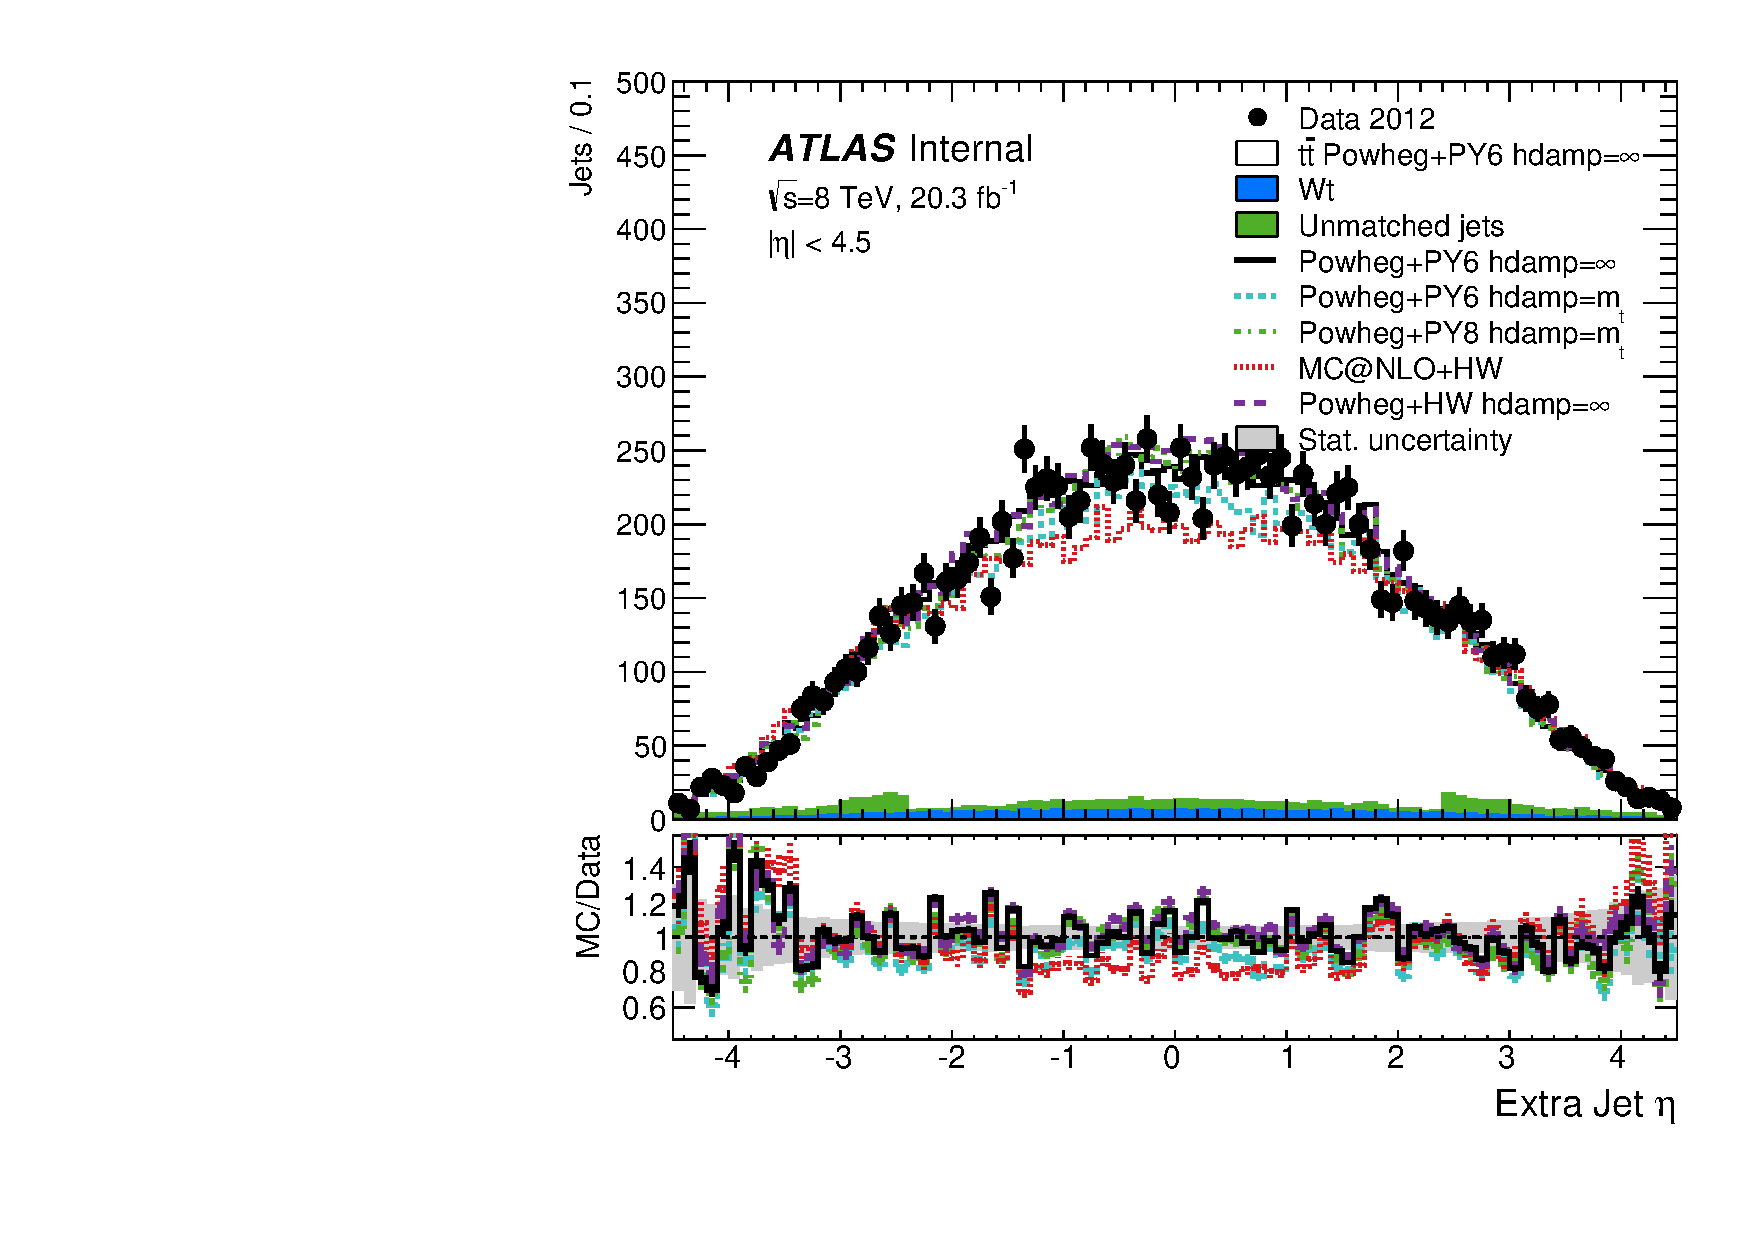
\includegraphics[width=0.9\textwidth]{fig/MCComp/NLO/ExtraJetEta.pdf}
\caption{The $\eta$ distribution of extra jets in simulation and data.}
\label{fig:jeteta}
\end{figure}

\begin{figure}
\subfloat[a]{
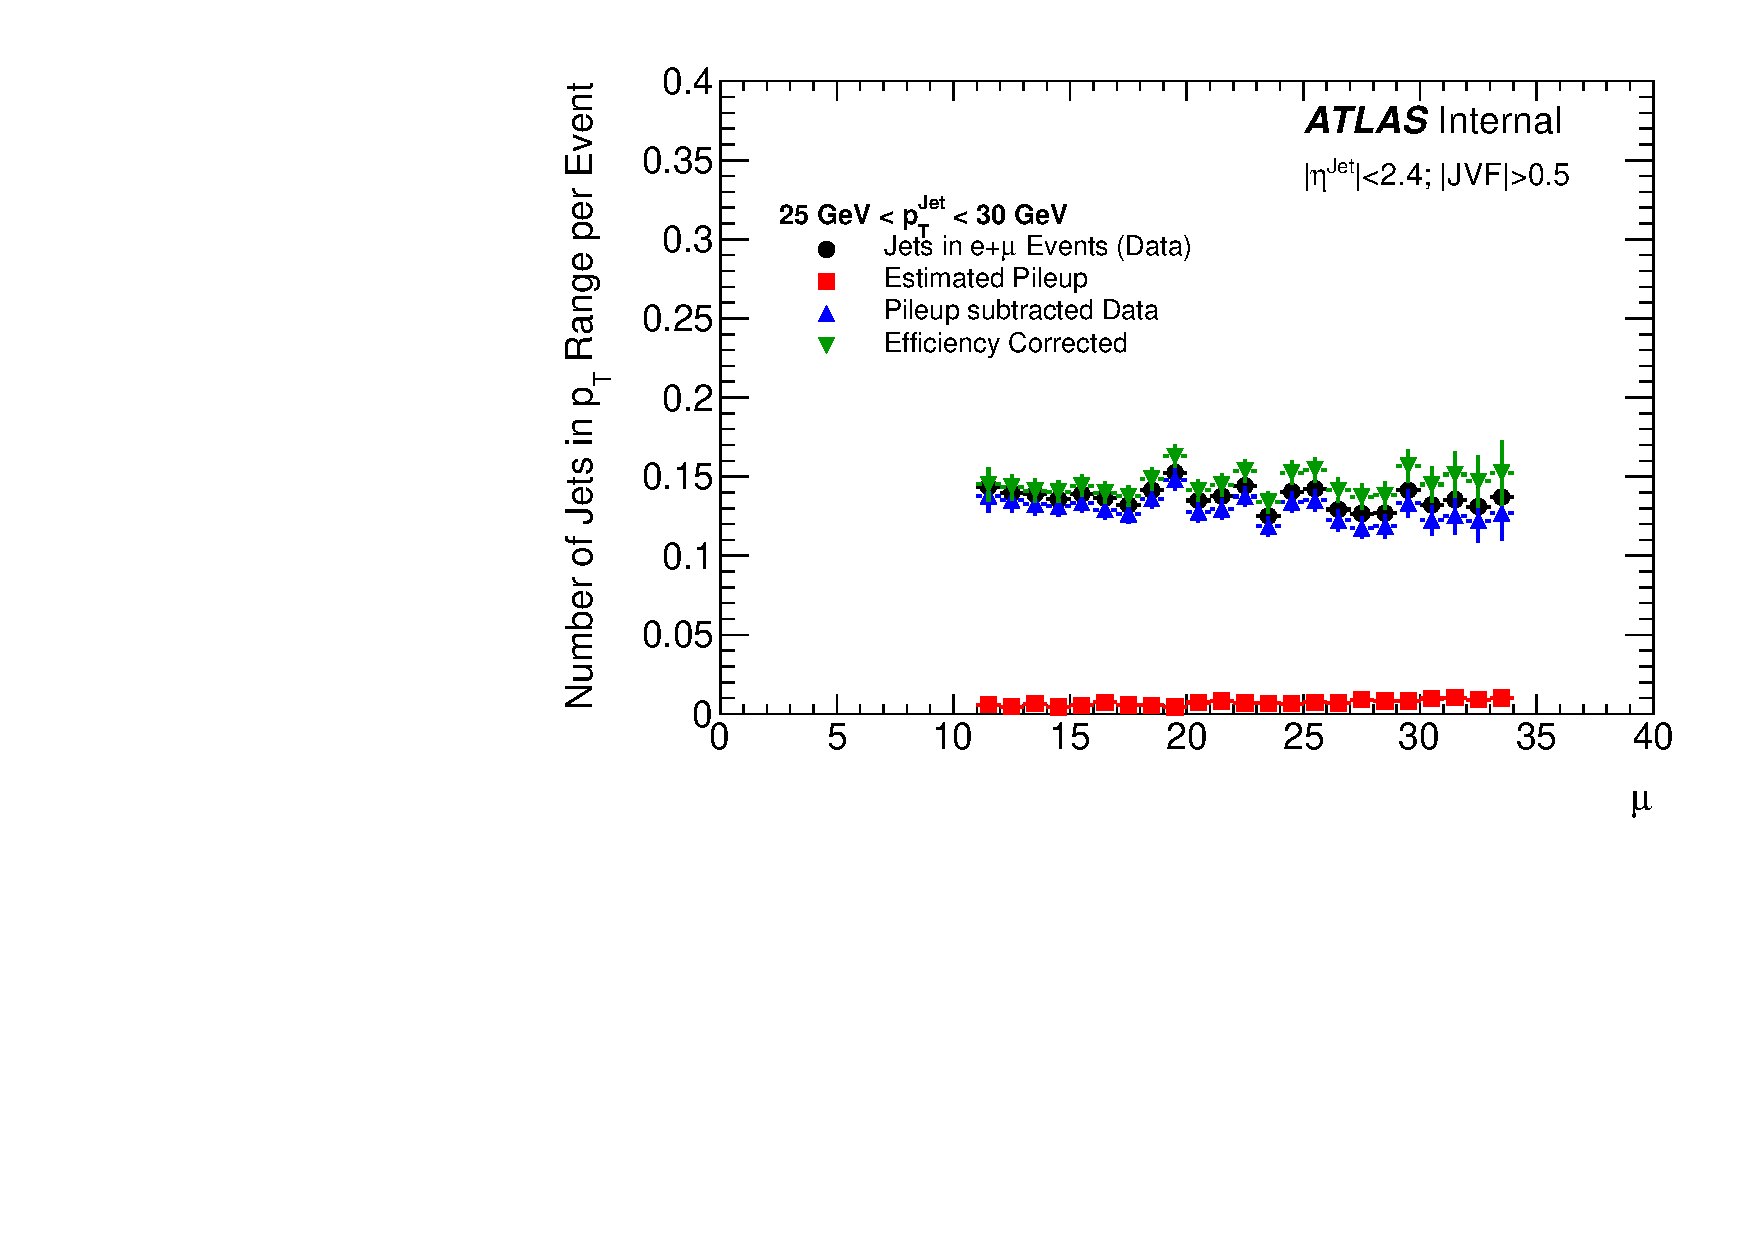
\includegraphics[width=0.48\textwidth]{fig/Pileup/EMuCentralJVF25_30_rates.pdf}}
\subfloat[b]{
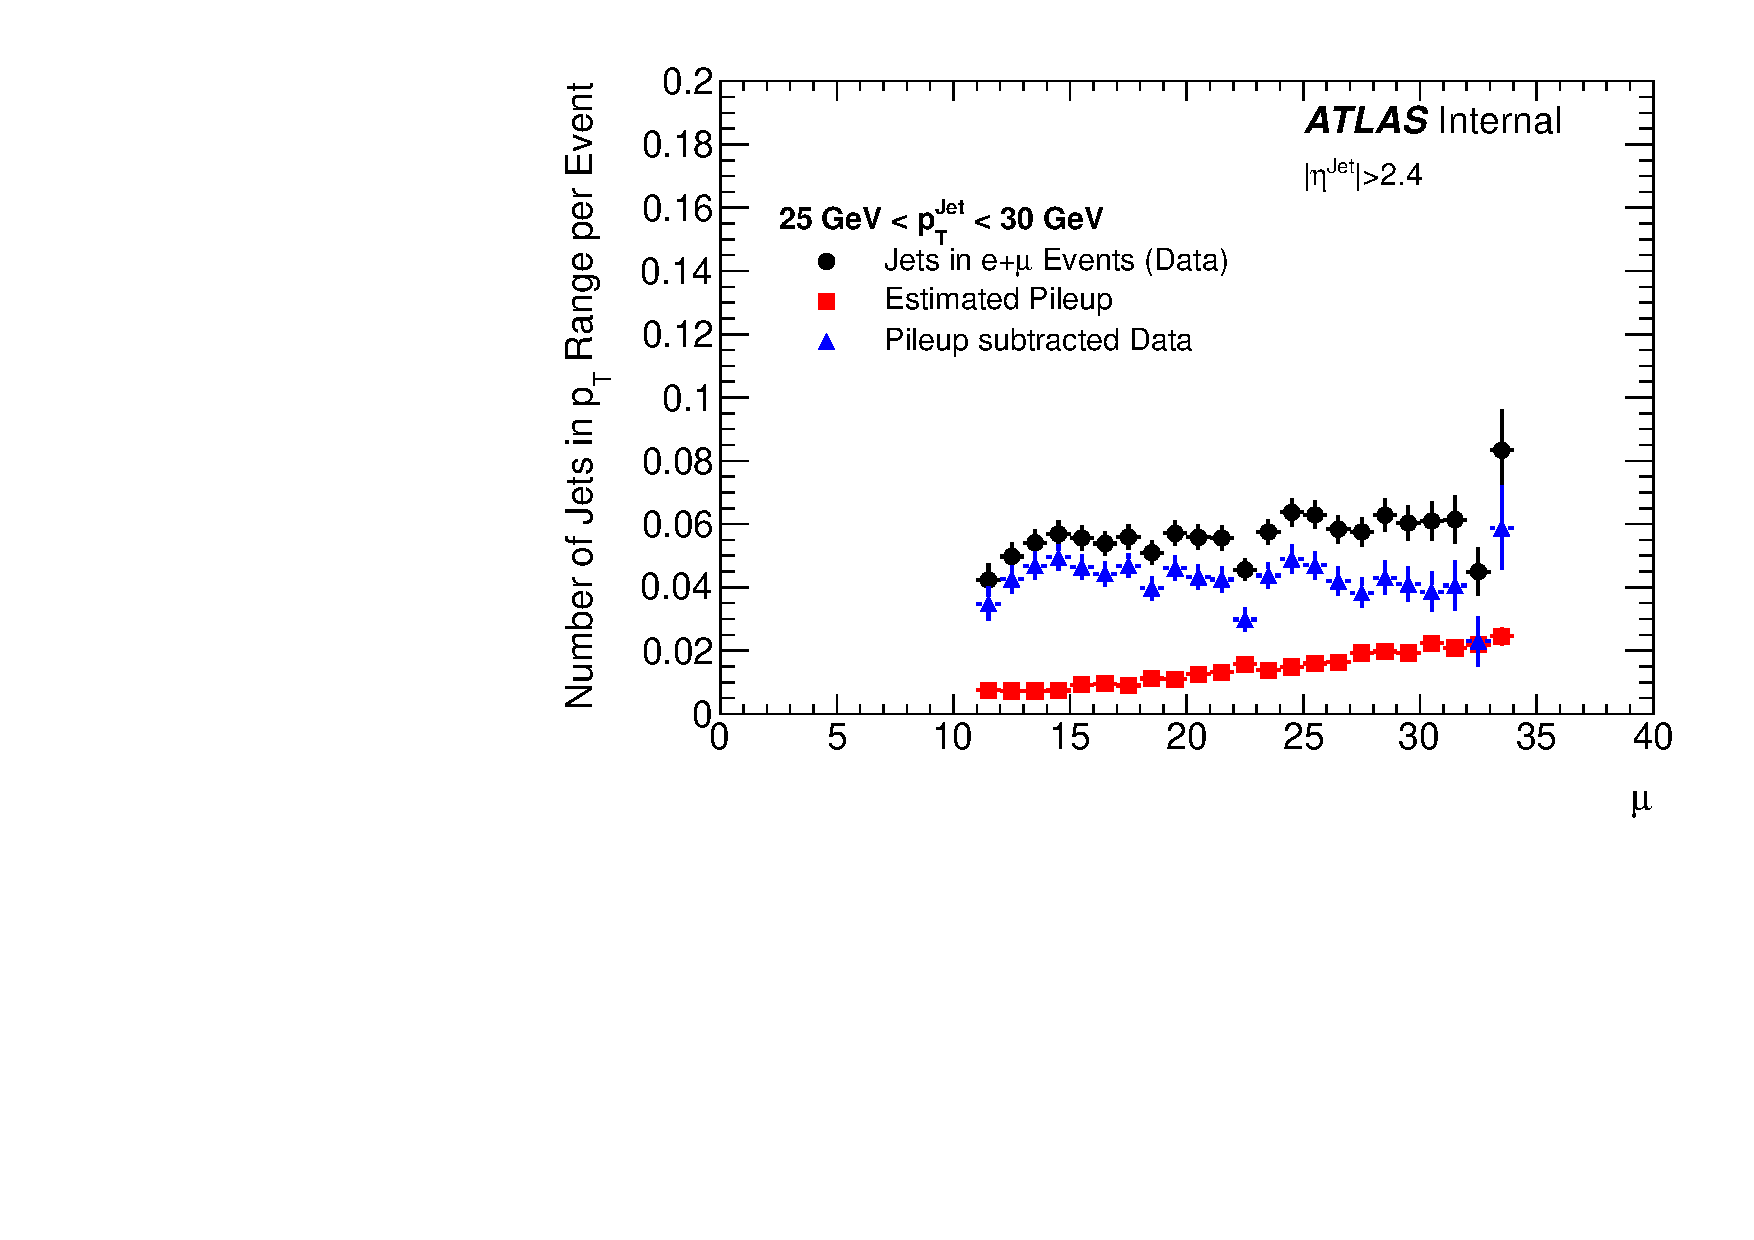
\includegraphics[width=0.48\textwidth]{fig/Pileup/EMuForward25_30_rates.pdf}}

\caption{Mean number of reconstructed jets as a function of $<\mu>$ 
for jets in the $p_T$~range $25<p_T<30$~GeV for (a) central and (b) forward jets
in data events passing the $e$-$\mu$ selection before and after correction for pileup.
Jets passing the 70\%\  MV1 b-tagging selection are removed.
The pileup rate is estimated using the ZeroBiasOverlay data stream.
The blue markers show the pileup subtracted rate before correcting
for the $<\mu>$-dependent efficiency of the JVF cut.  The green
points show the results after correction.}
\label{fig:pileupjets}
\end{figure}

\begin{figure}
\centering
\subfloat{
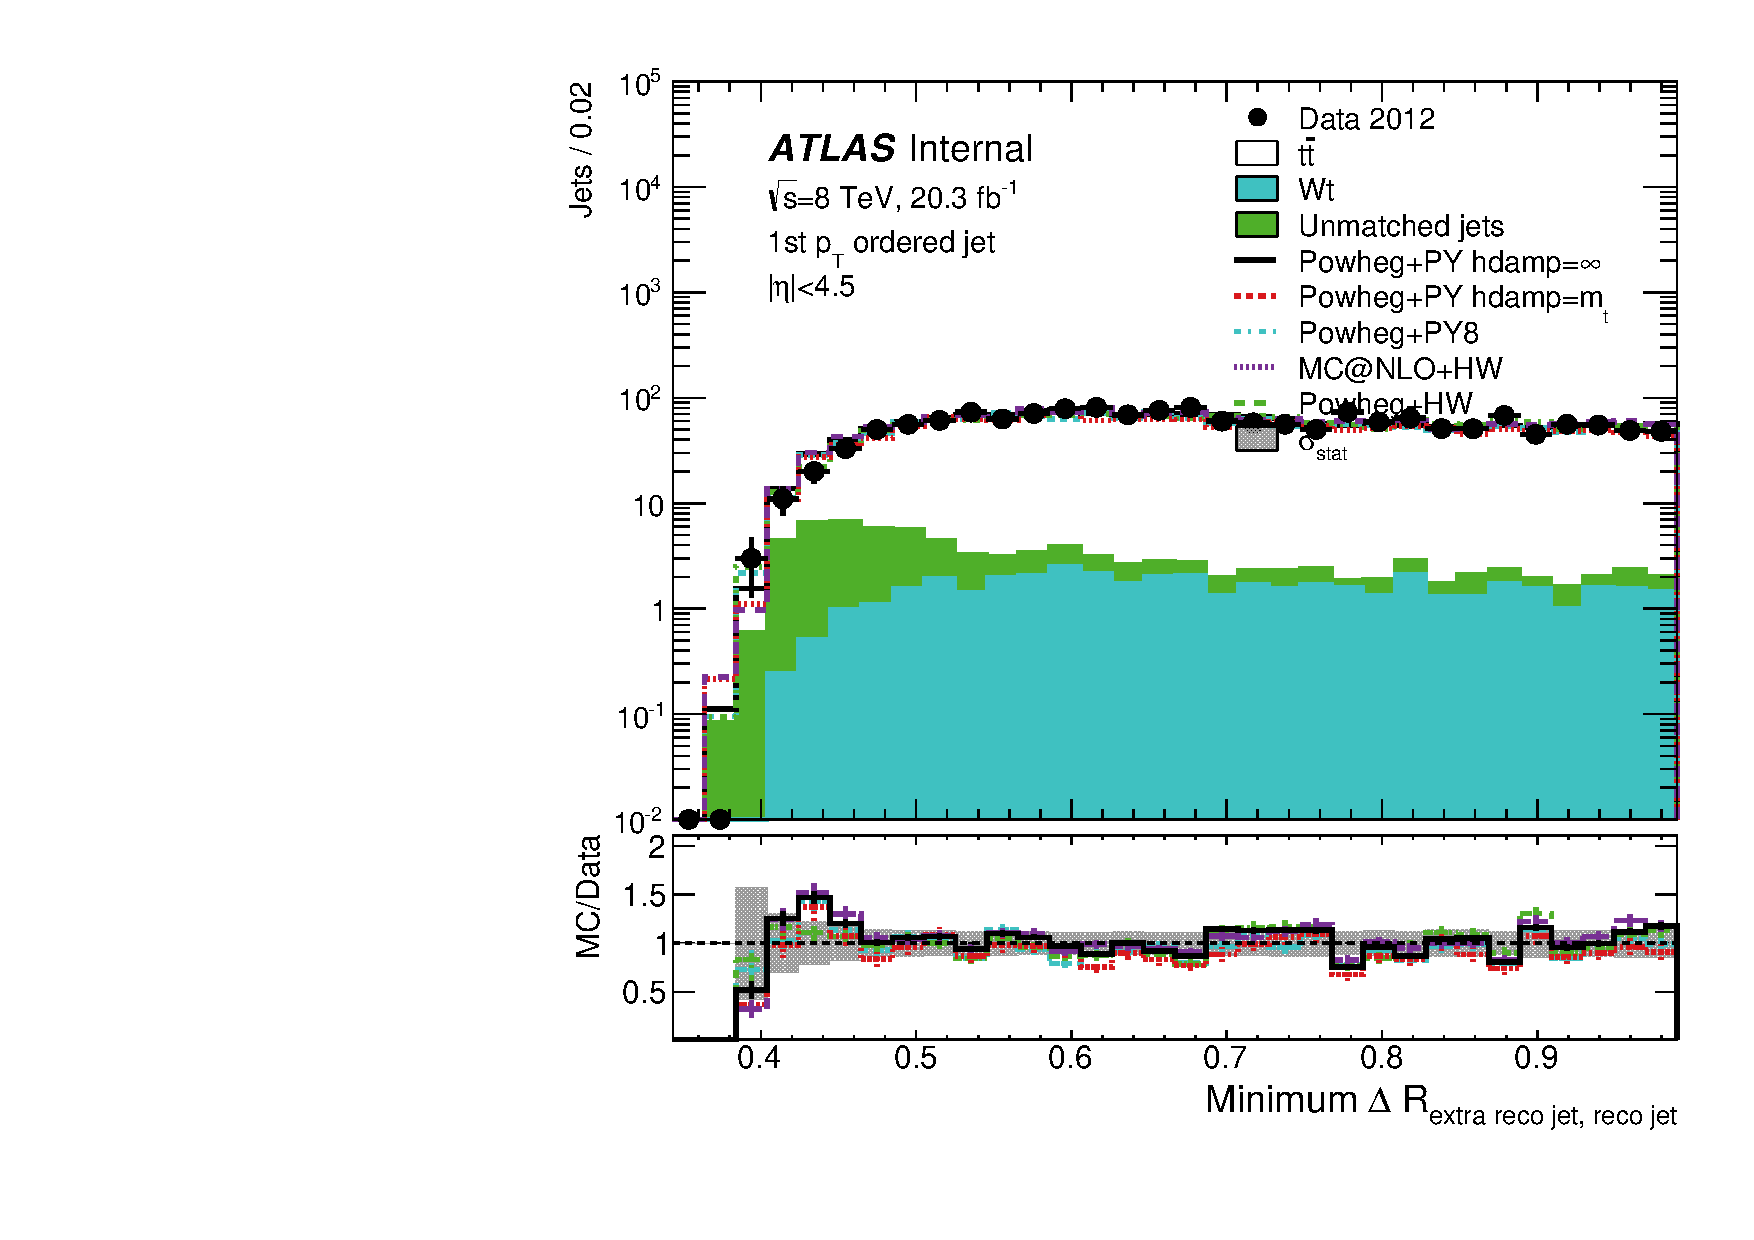
\includegraphics[width=0.45\textwidth]{fig/MCComp/NLO/GrandPtVsRecoDRJet0.pdf}}
\subfloat{
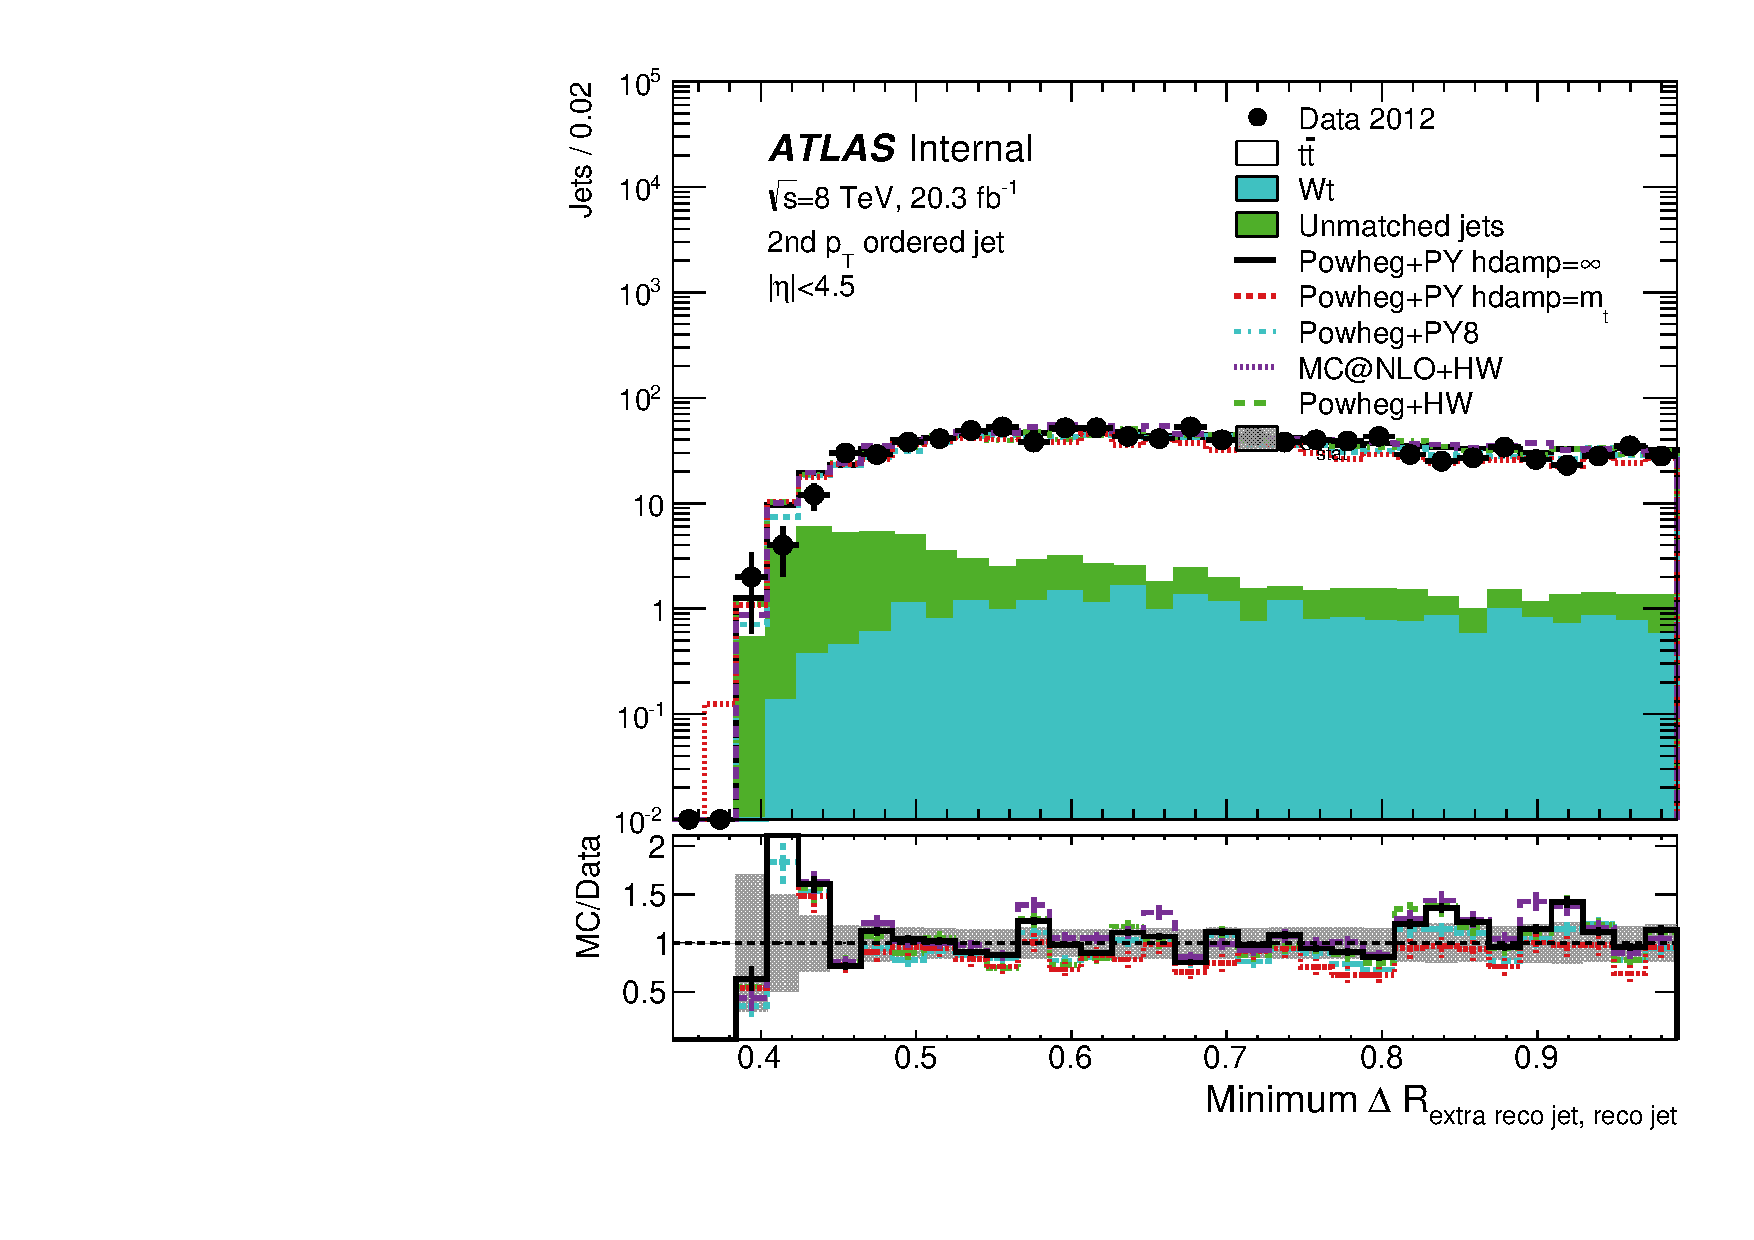
\includegraphics[width=0.45\textwidth]{fig/MCComp/NLO/GrandPtVsRecoDRJet1.pdf}}
\\
\subfloat{
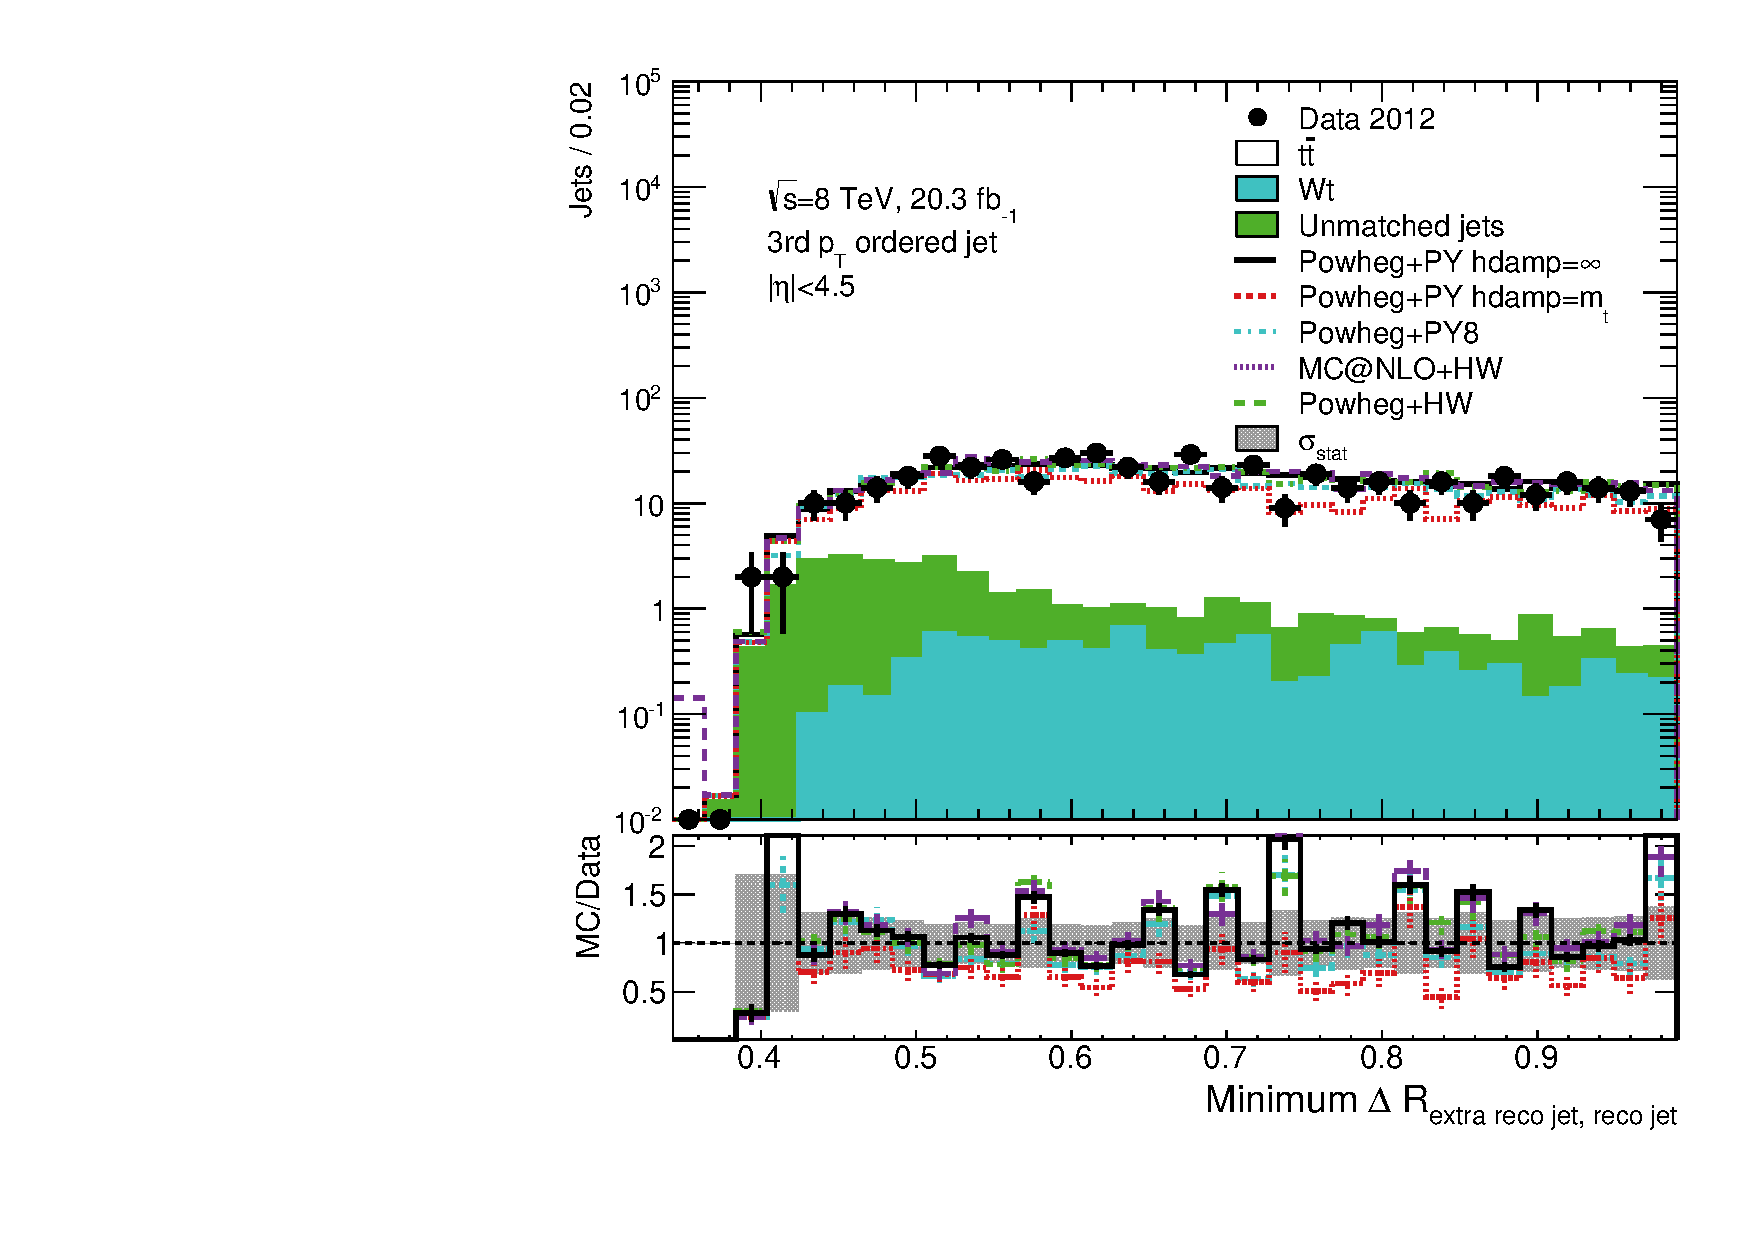
\includegraphics[width=0.45\textwidth]{fig/MCComp/NLO/GrandPtVsRecoDRJet2.pdf}}
\subfloat{
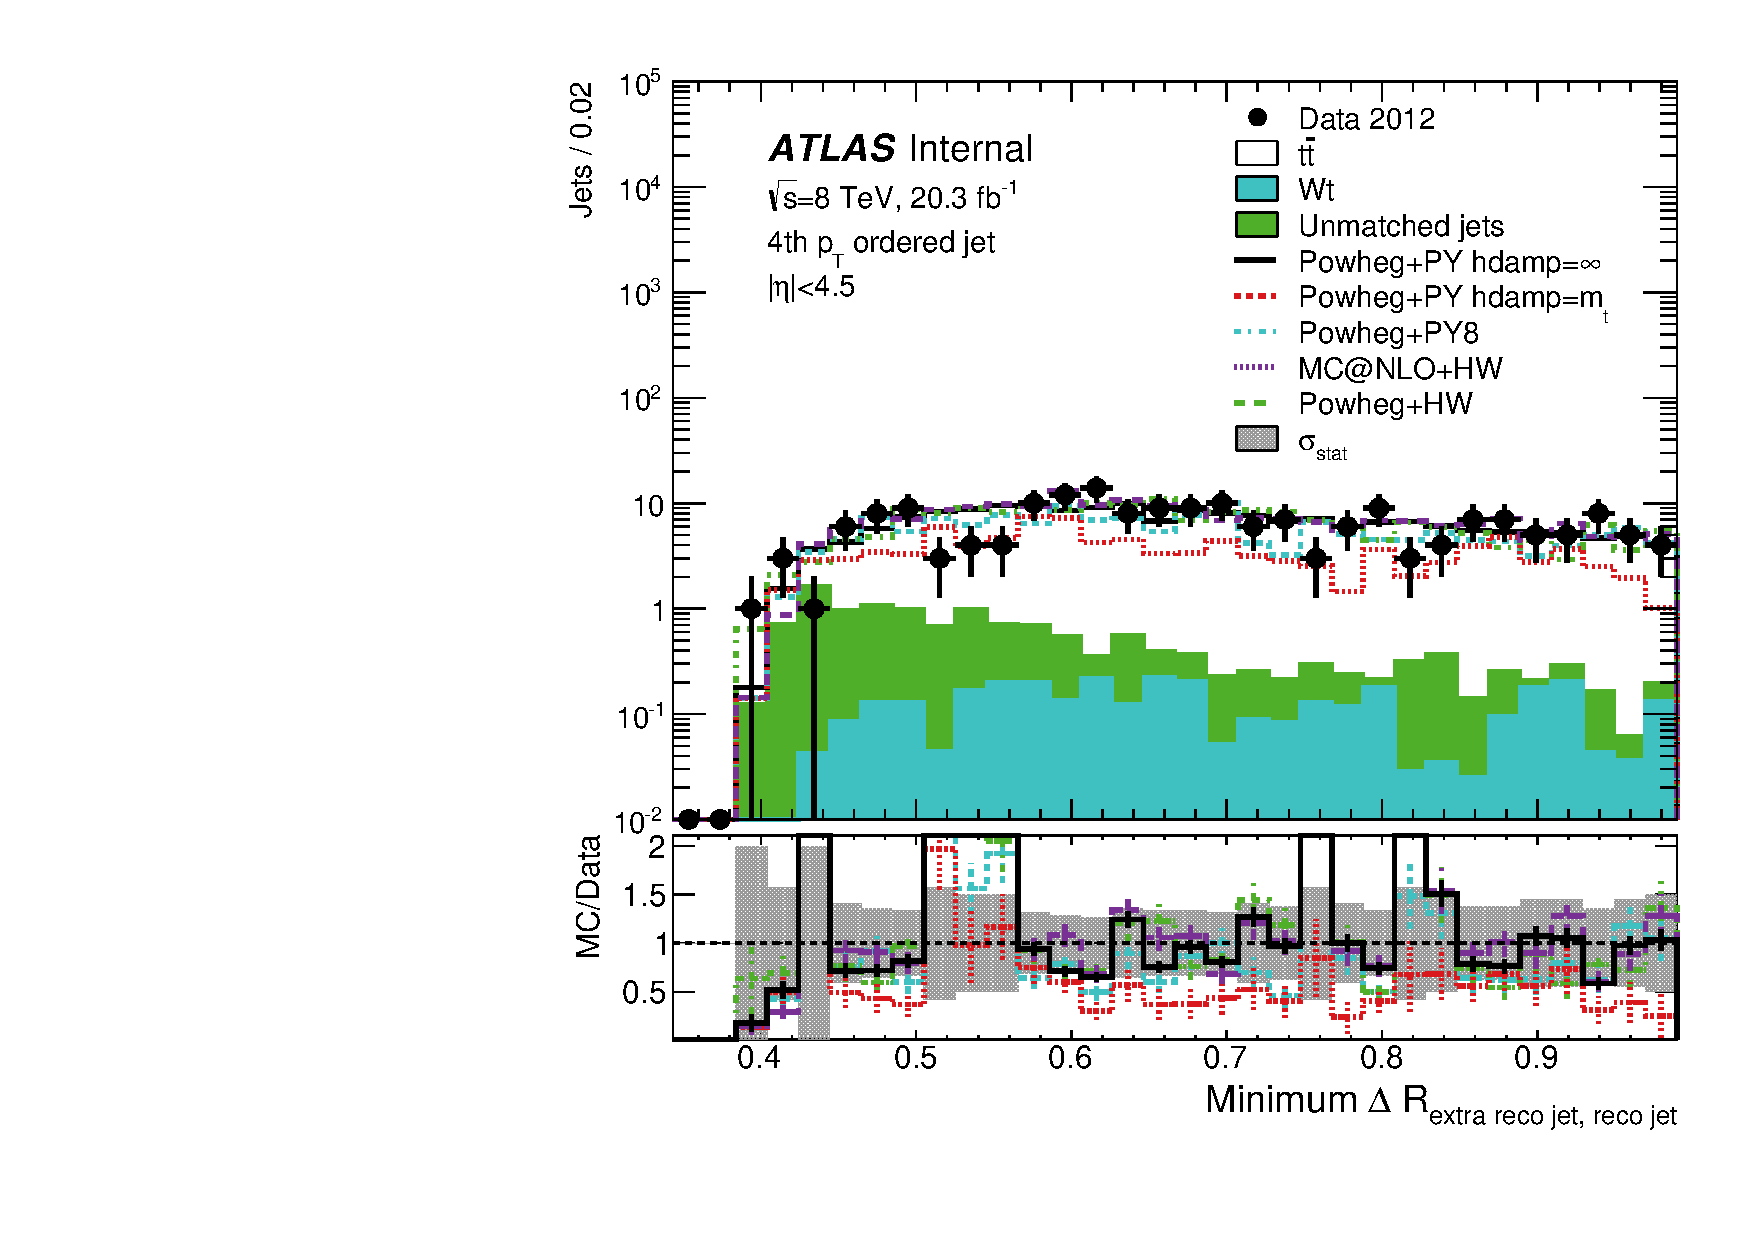
\includegraphics[width=0.45\textwidth]{fig/MCComp/NLO/GrandPtVsRecoDRJet3.pdf}}
\caption{Distributions of minimum reconstructed $\Delta R$ betweeen extra jets in simulation and data for the the first, second, third and fourth extra jet. }
\label{fig:recodr}
\end{figure}
\begin{figure}
\centering
\subfloat{
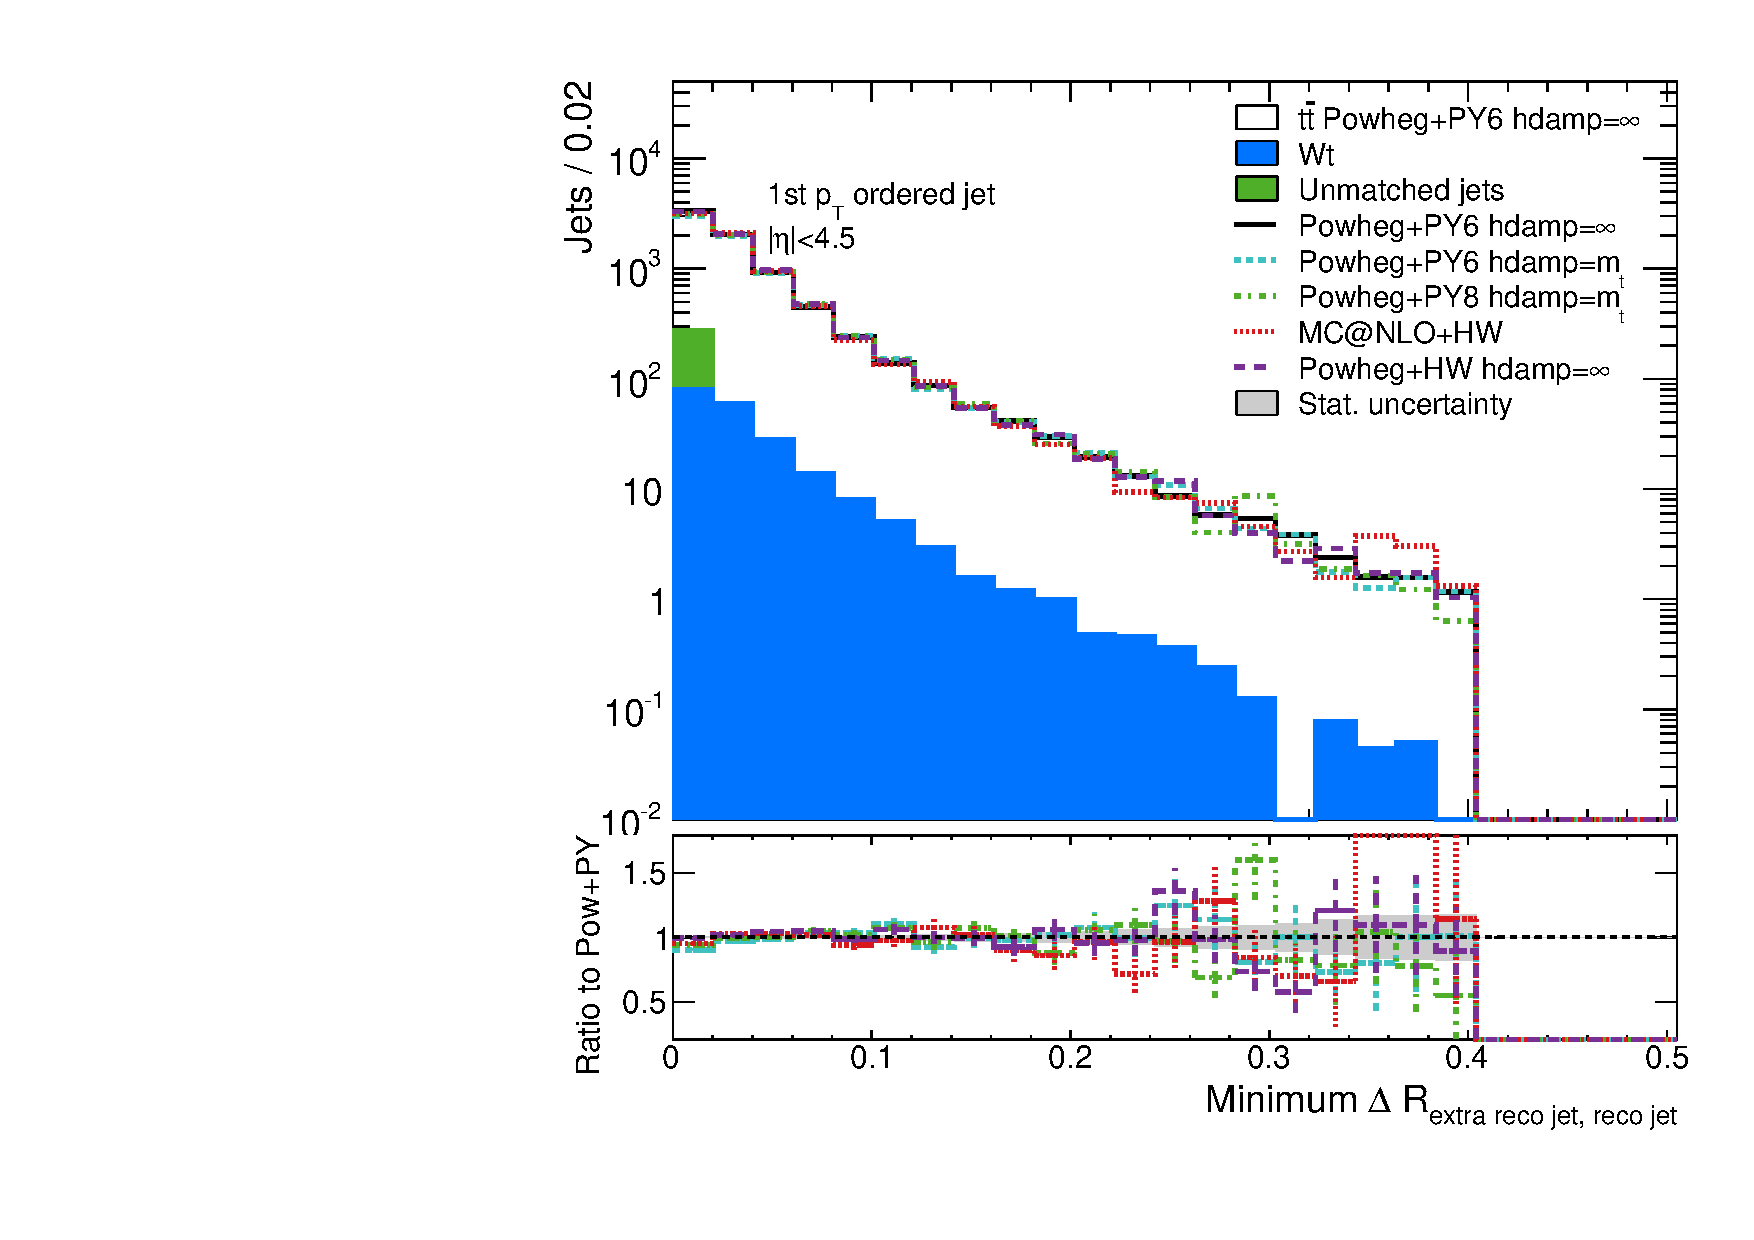
\includegraphics[width=0.45\textwidth]{fig/MCComp/NLO/GrandPtVsTruthDRJet0.pdf}}
\subfloat{
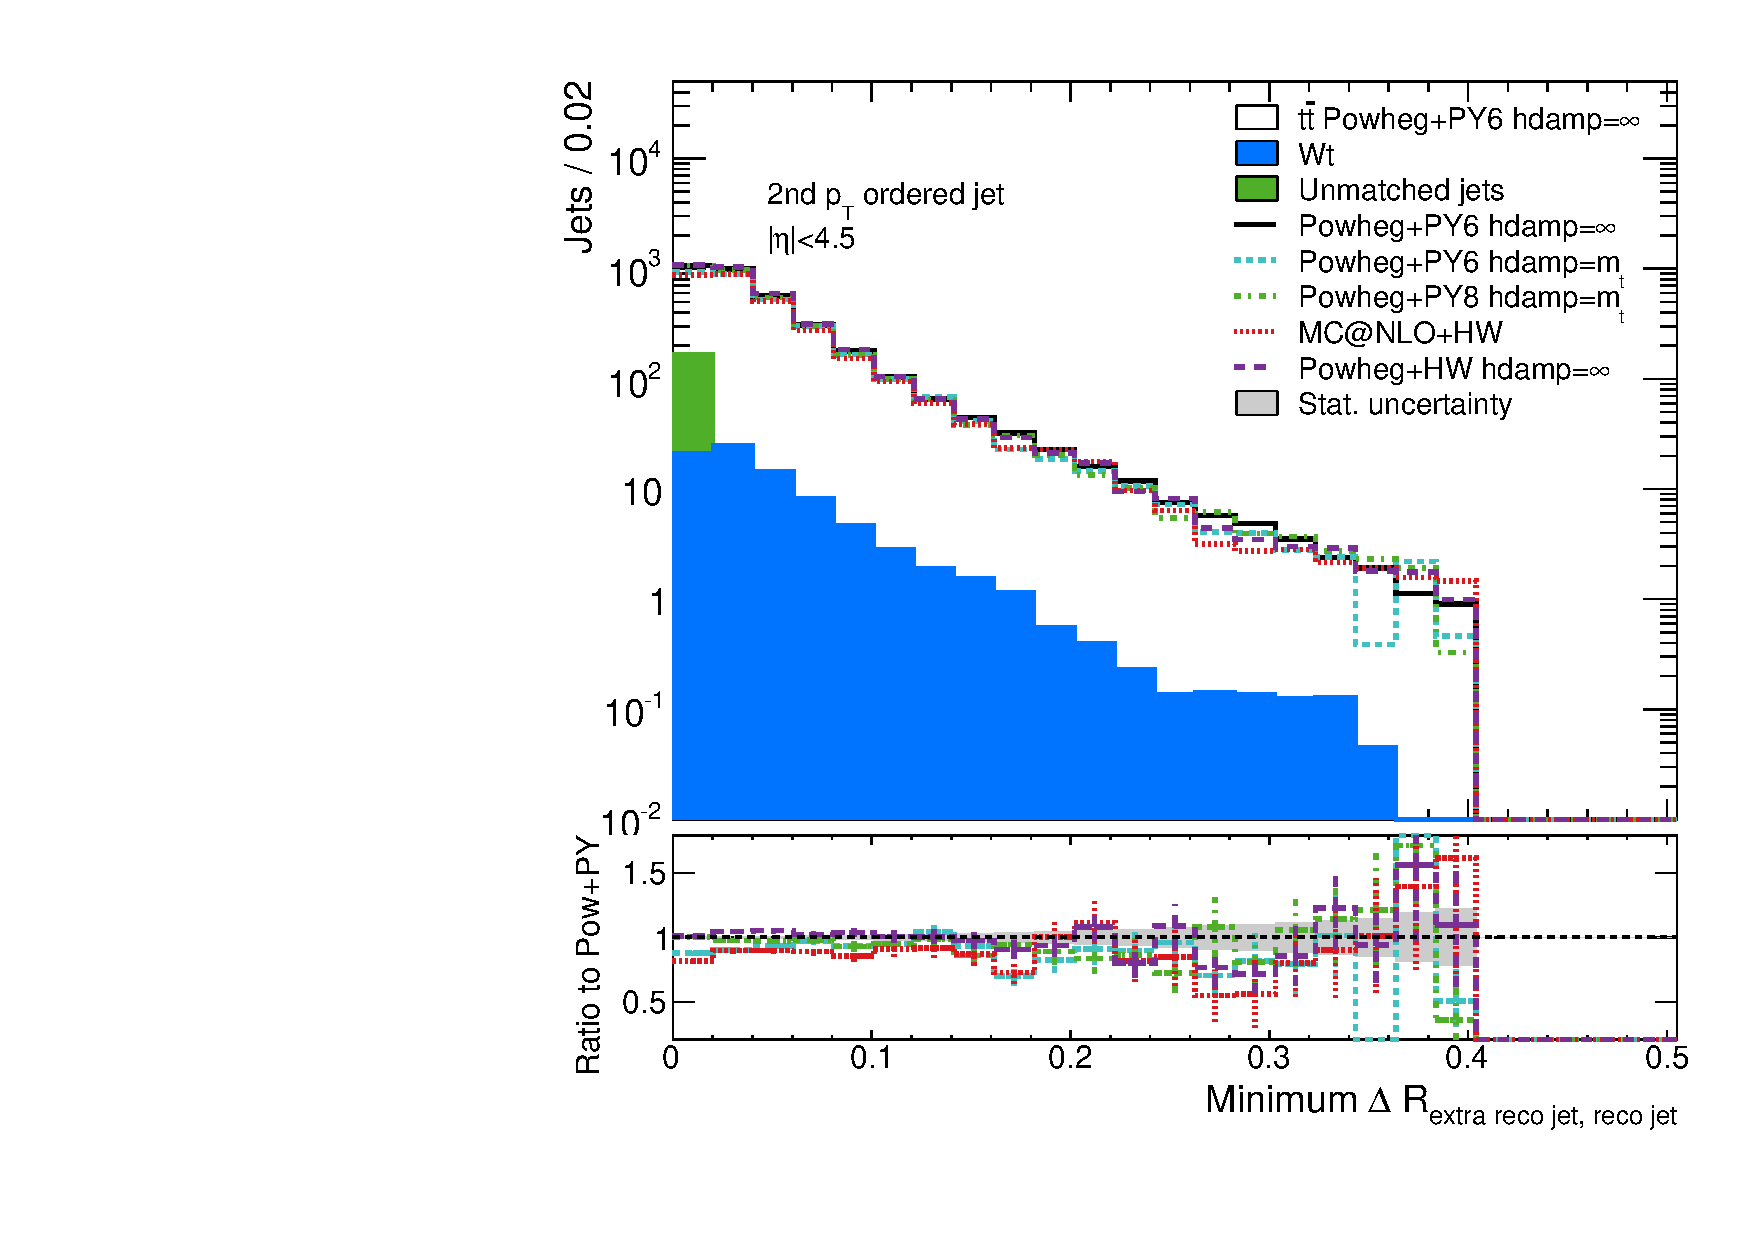
\includegraphics[width=0.45\textwidth]{fig/MCComp/NLO/GrandPtVsTruthDRJet1.pdf}}
\\
\subfloat{
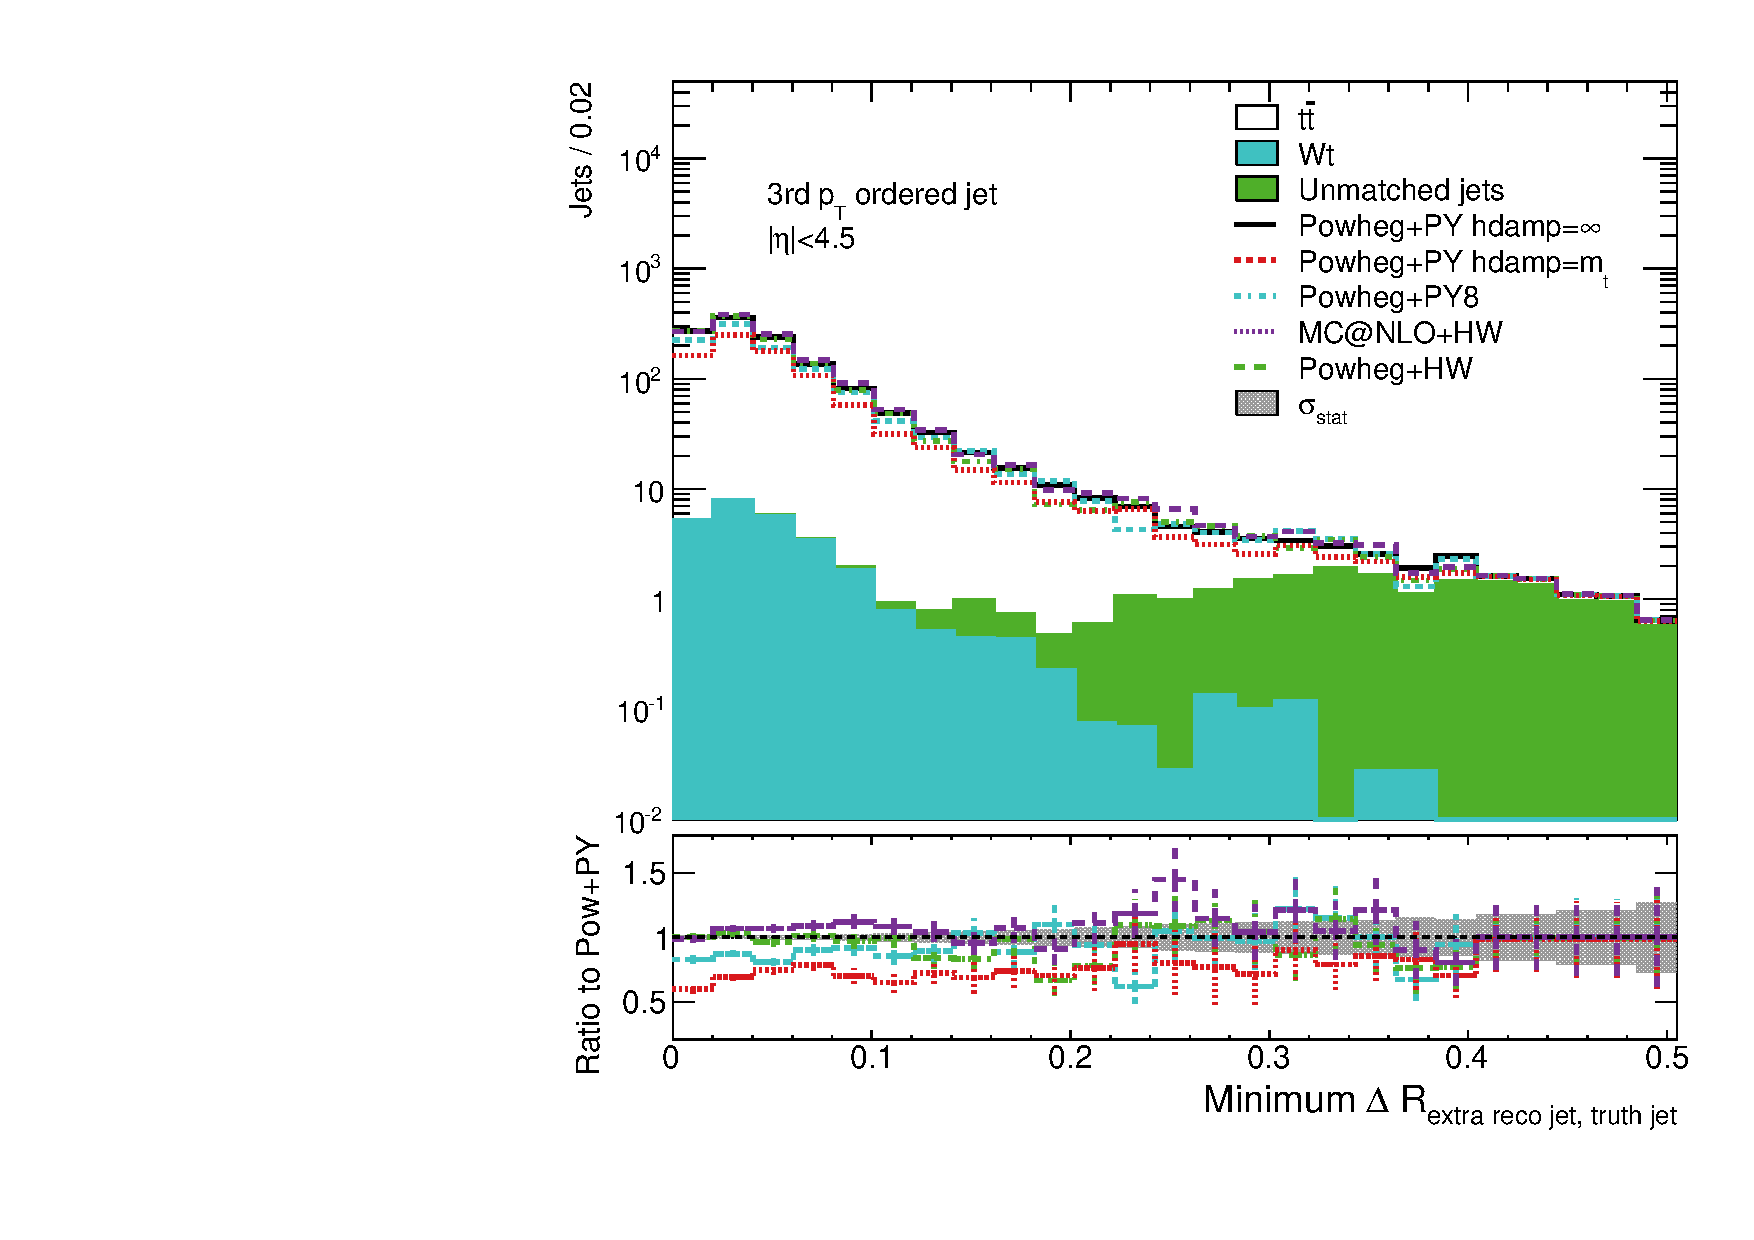
\includegraphics[width=0.45\textwidth]{fig/MCComp/NLO/GrandPtVsTruthDRJet2.pdf}}
\subfloat{
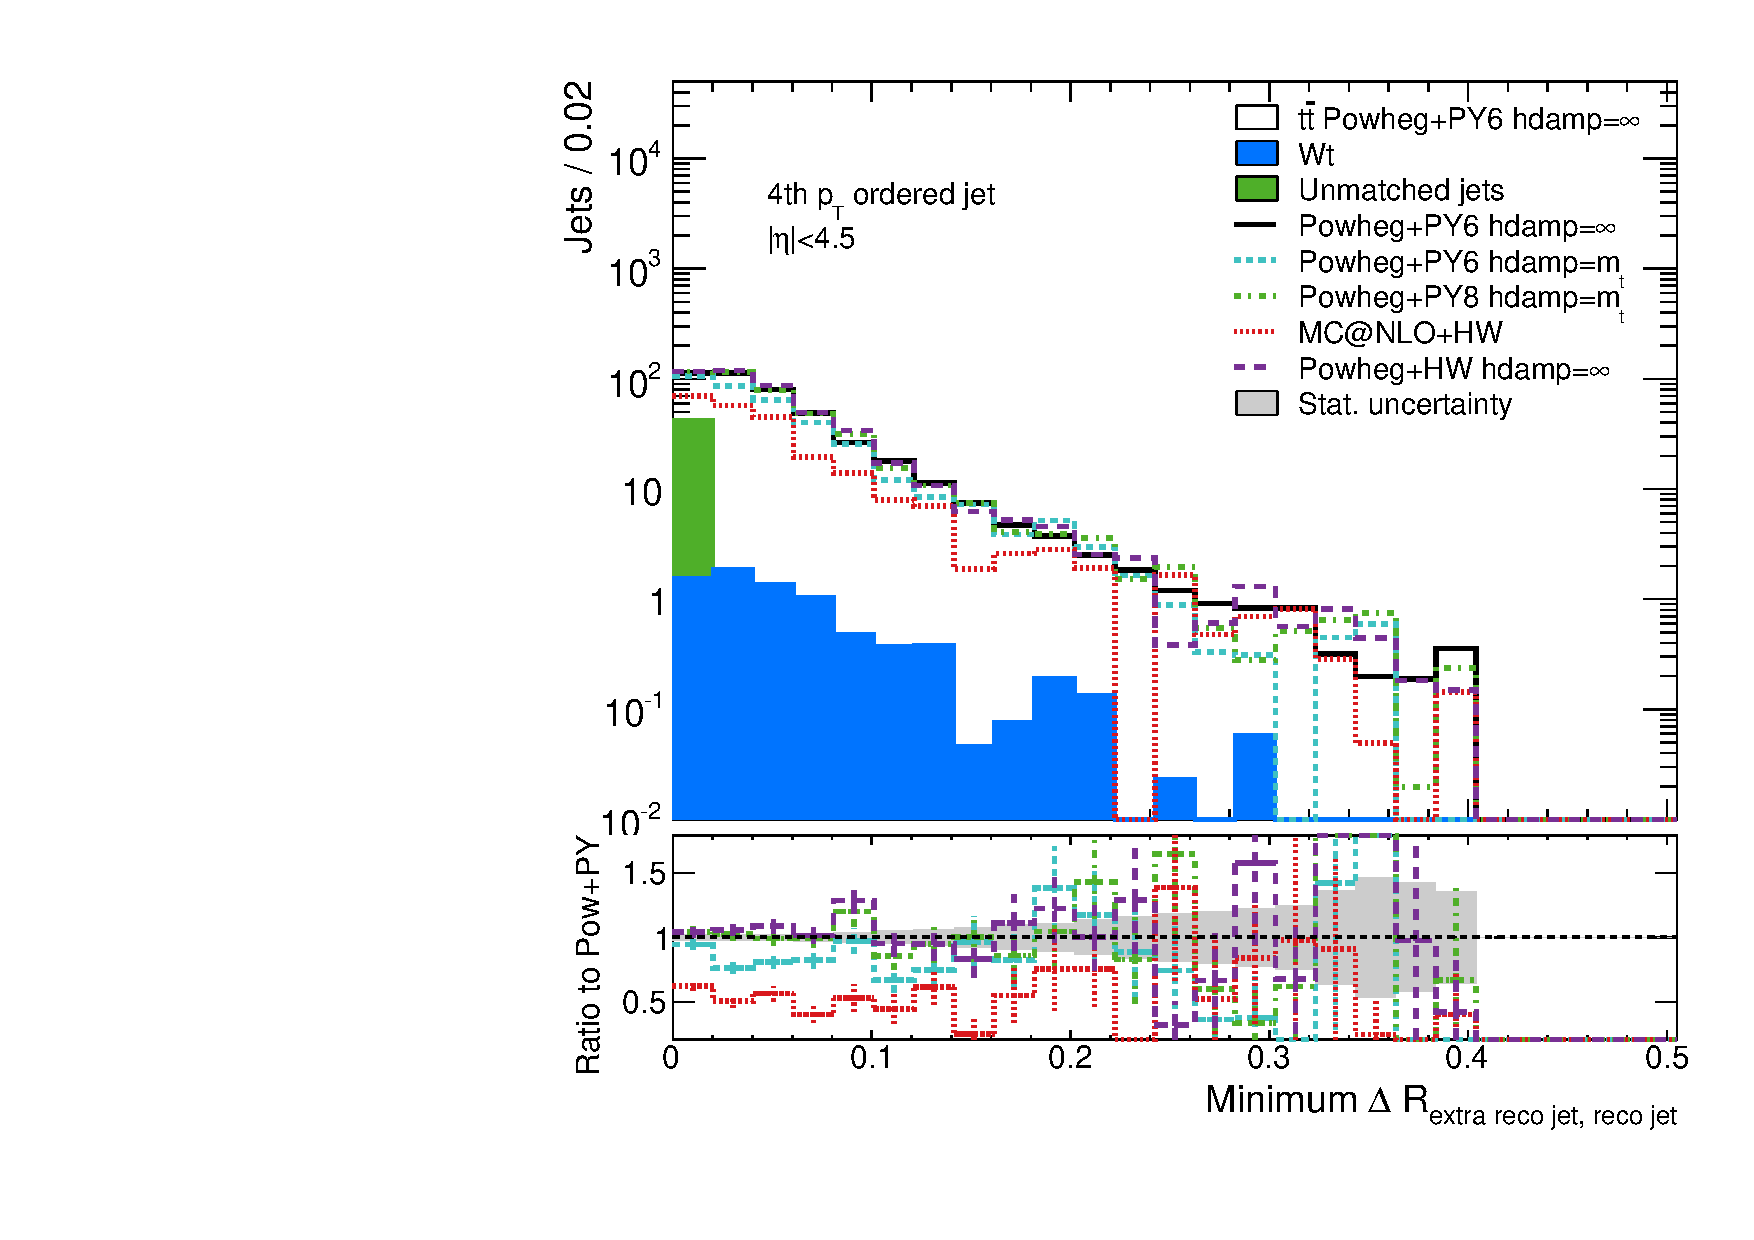
\includegraphics[width=0.45\textwidth]{fig/MCComp/NLO/GrandPtVsTruthDRJet3.pdf}}
\caption{Distributions of $\Delta R$ betweeen reconstructed extra jets and the nearest truth jet for the first, second, third and fourth extra jet. }
\label{fig:truthdr}
\end{figure}
\section{Reconstruction level distributions}

Figures~\ref{fig:nrecojets} and~\ref{fig:recojetpt} compare the multiplicity and \pt of reconstructed extra jets in data and \ttbar simulation, where the simulation has been normalized to the number of events in data. Statistical uncertainity on the data is shown as a gray band on the ratio plot and statistical uncertainty on the simulation is shown as a error bars on the ratio.  Systematic uncertainities are not shown. 
%For both the simulation and the data in Figure~\ref{fig:nrecojets}, jets from pileup are not included. 
%Pileup and false jet backgrounds have been removed from both the data and the simulation.
In data, background from pileup jets is subtracted, while in simulation, reconstructed jets are required to have a truth match. The multiplicity 
in the MC samples agree with that of the data, except for \mcnlohw, which consistently underestimates the number of events with 3 or more extra jets. Figure~\ref{fig:recojetpt} shows the \pt distributions of each extra jet, including contributions from single top events and unmatched jets. 
The fact that \mcnlohw\ underestimates the jet multiplicity can be seen in these distributions. The jets in \peight\ appear to exhibit a slightly harder spectrum than the data. All other generators agree reasonably well with the data. 
\begin{figure}
\centering
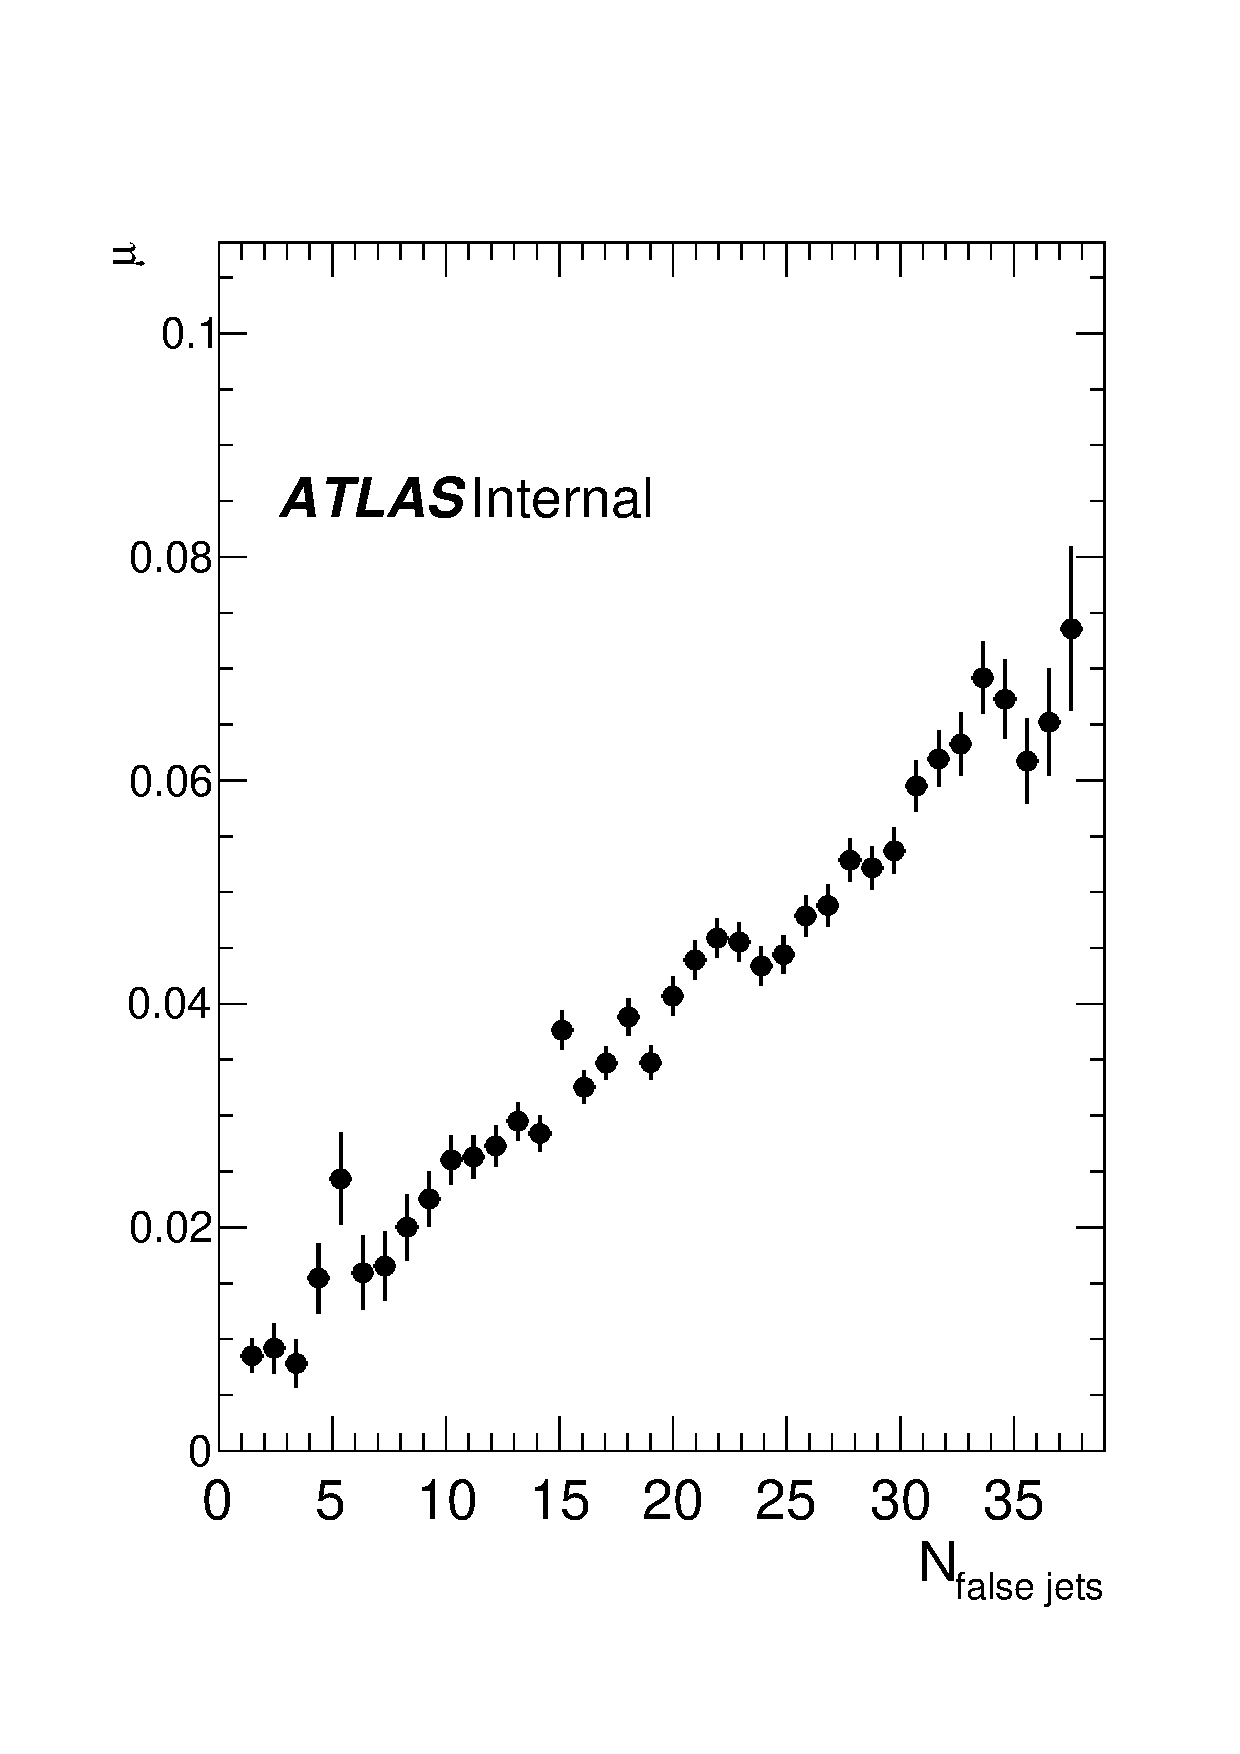
\includegraphics[width=0.45\textwidth]{fig/MCComp/FalseVsMu.pdf}
\caption{Dependence of the unmatched extra jet rate on $\mu$ for the baseline simulation.}
\label{fig:falsecomp}
\end{figure}

\begin{figure}
\centering
\subfloat{
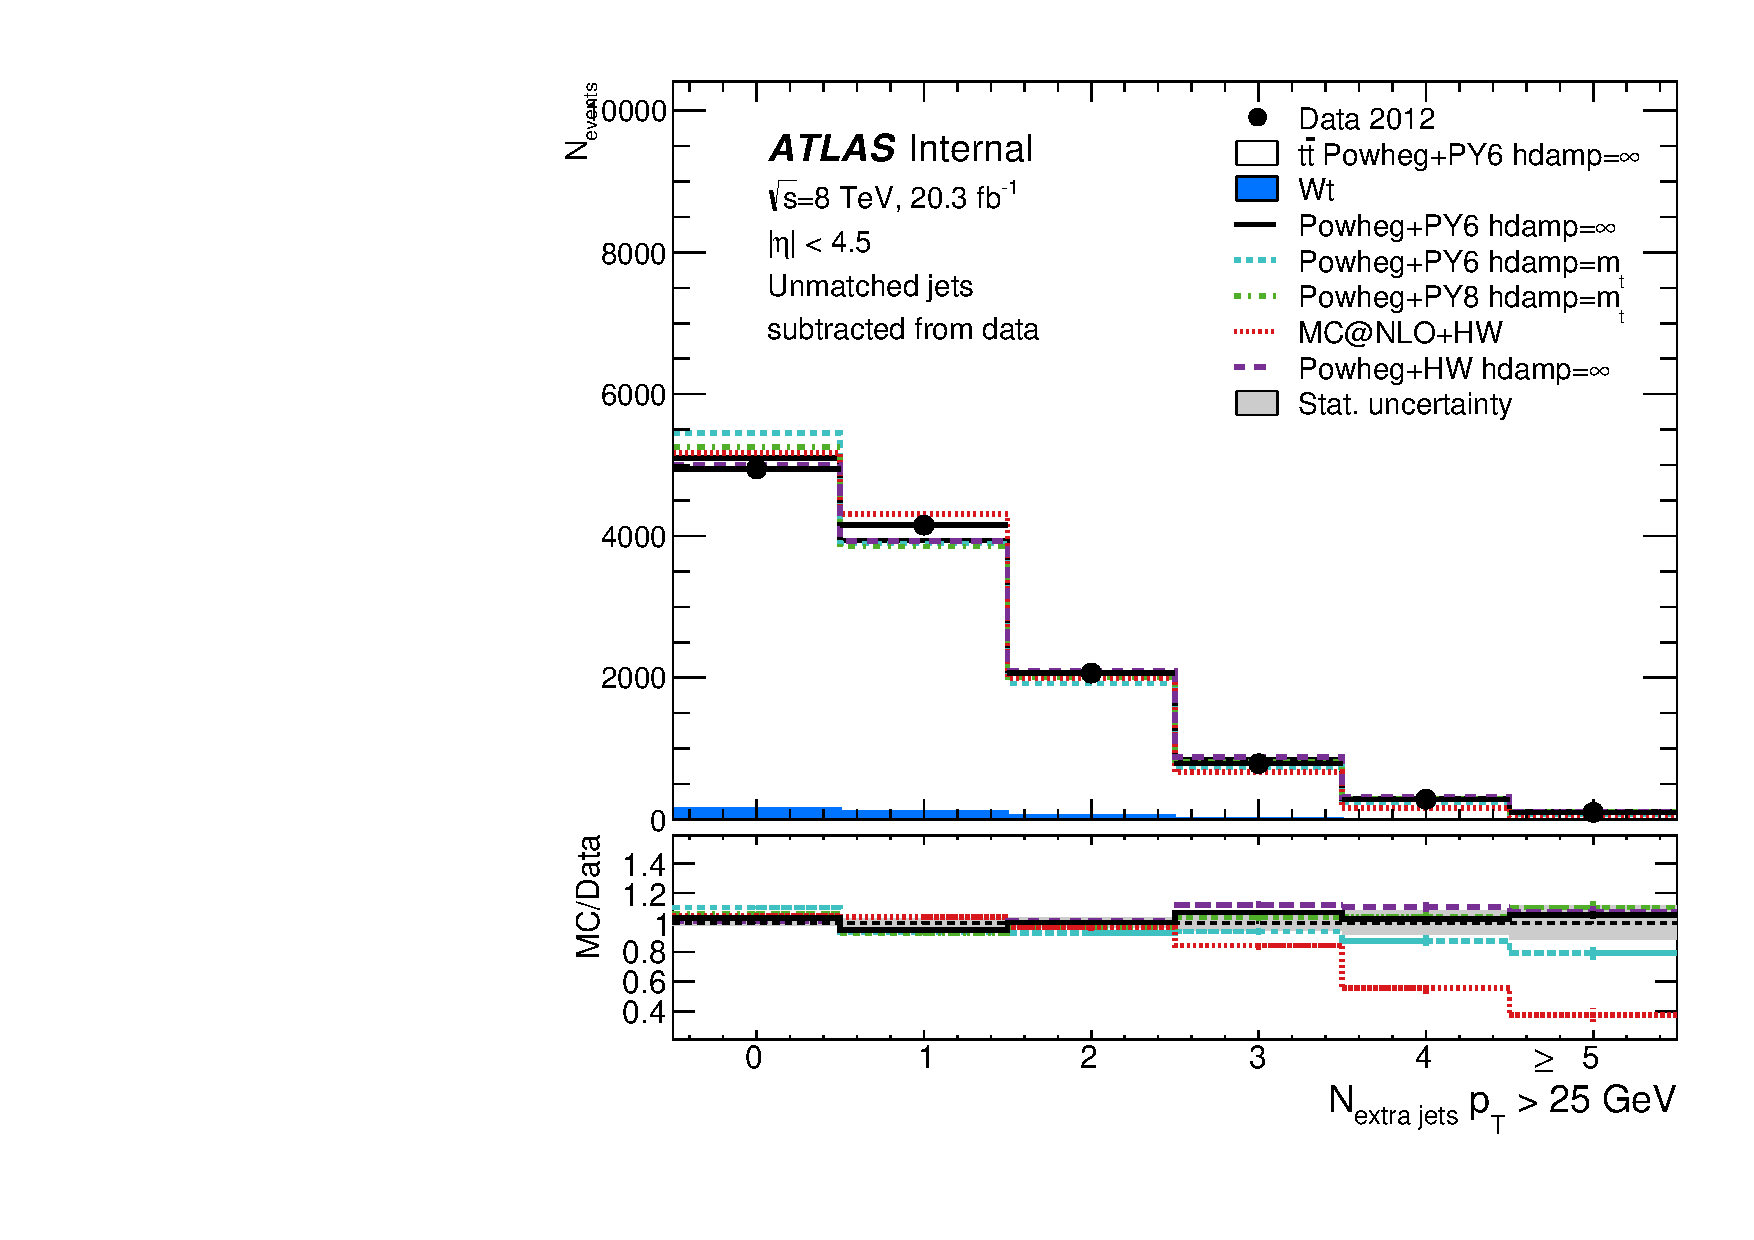
\includegraphics[width=0.45\textwidth]{fig/MCComp/NLO/NExtraJets25NoPileup.pdf}}
\subfloat{
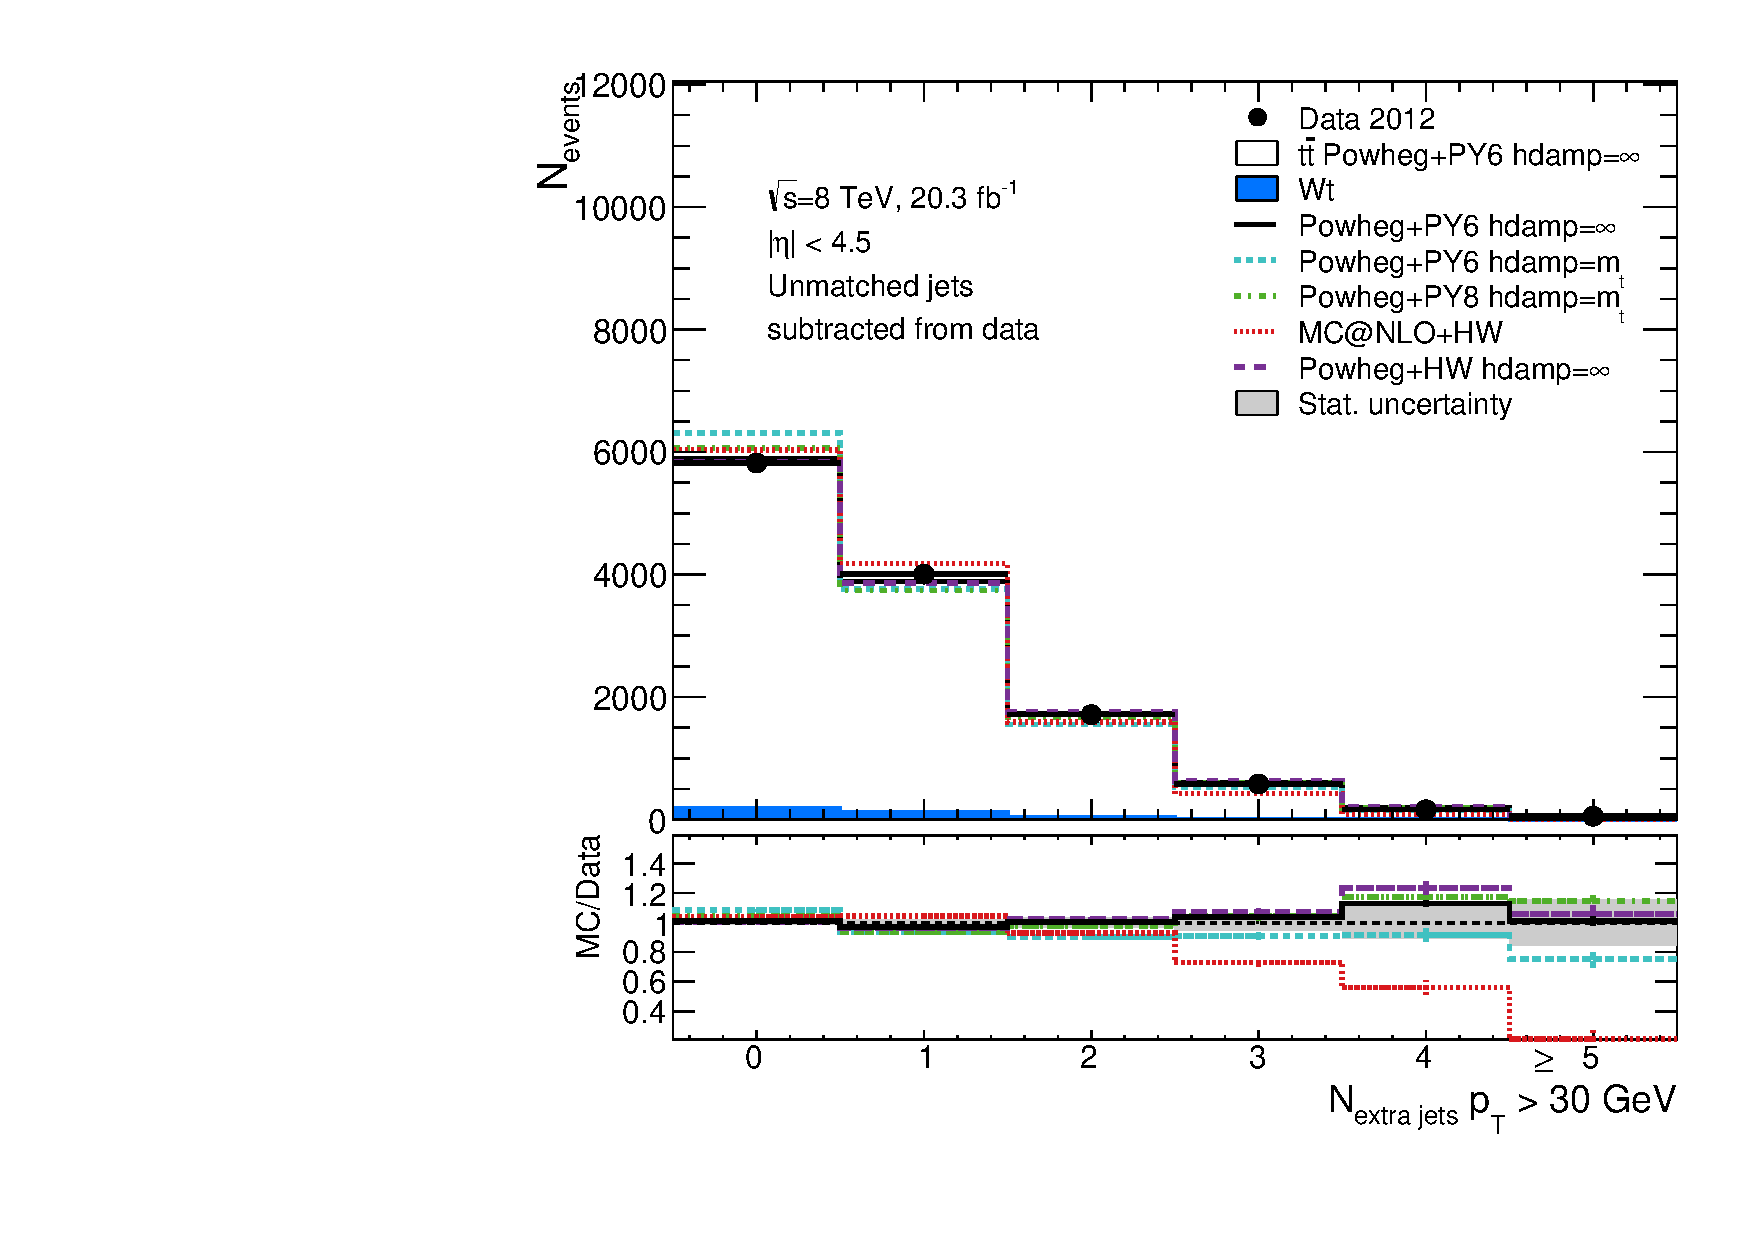
\includegraphics[width=0.45\textwidth]{fig/MCComp/NLO/NExtraJets30NoPileup.pdf}}
\\
\subfloat{
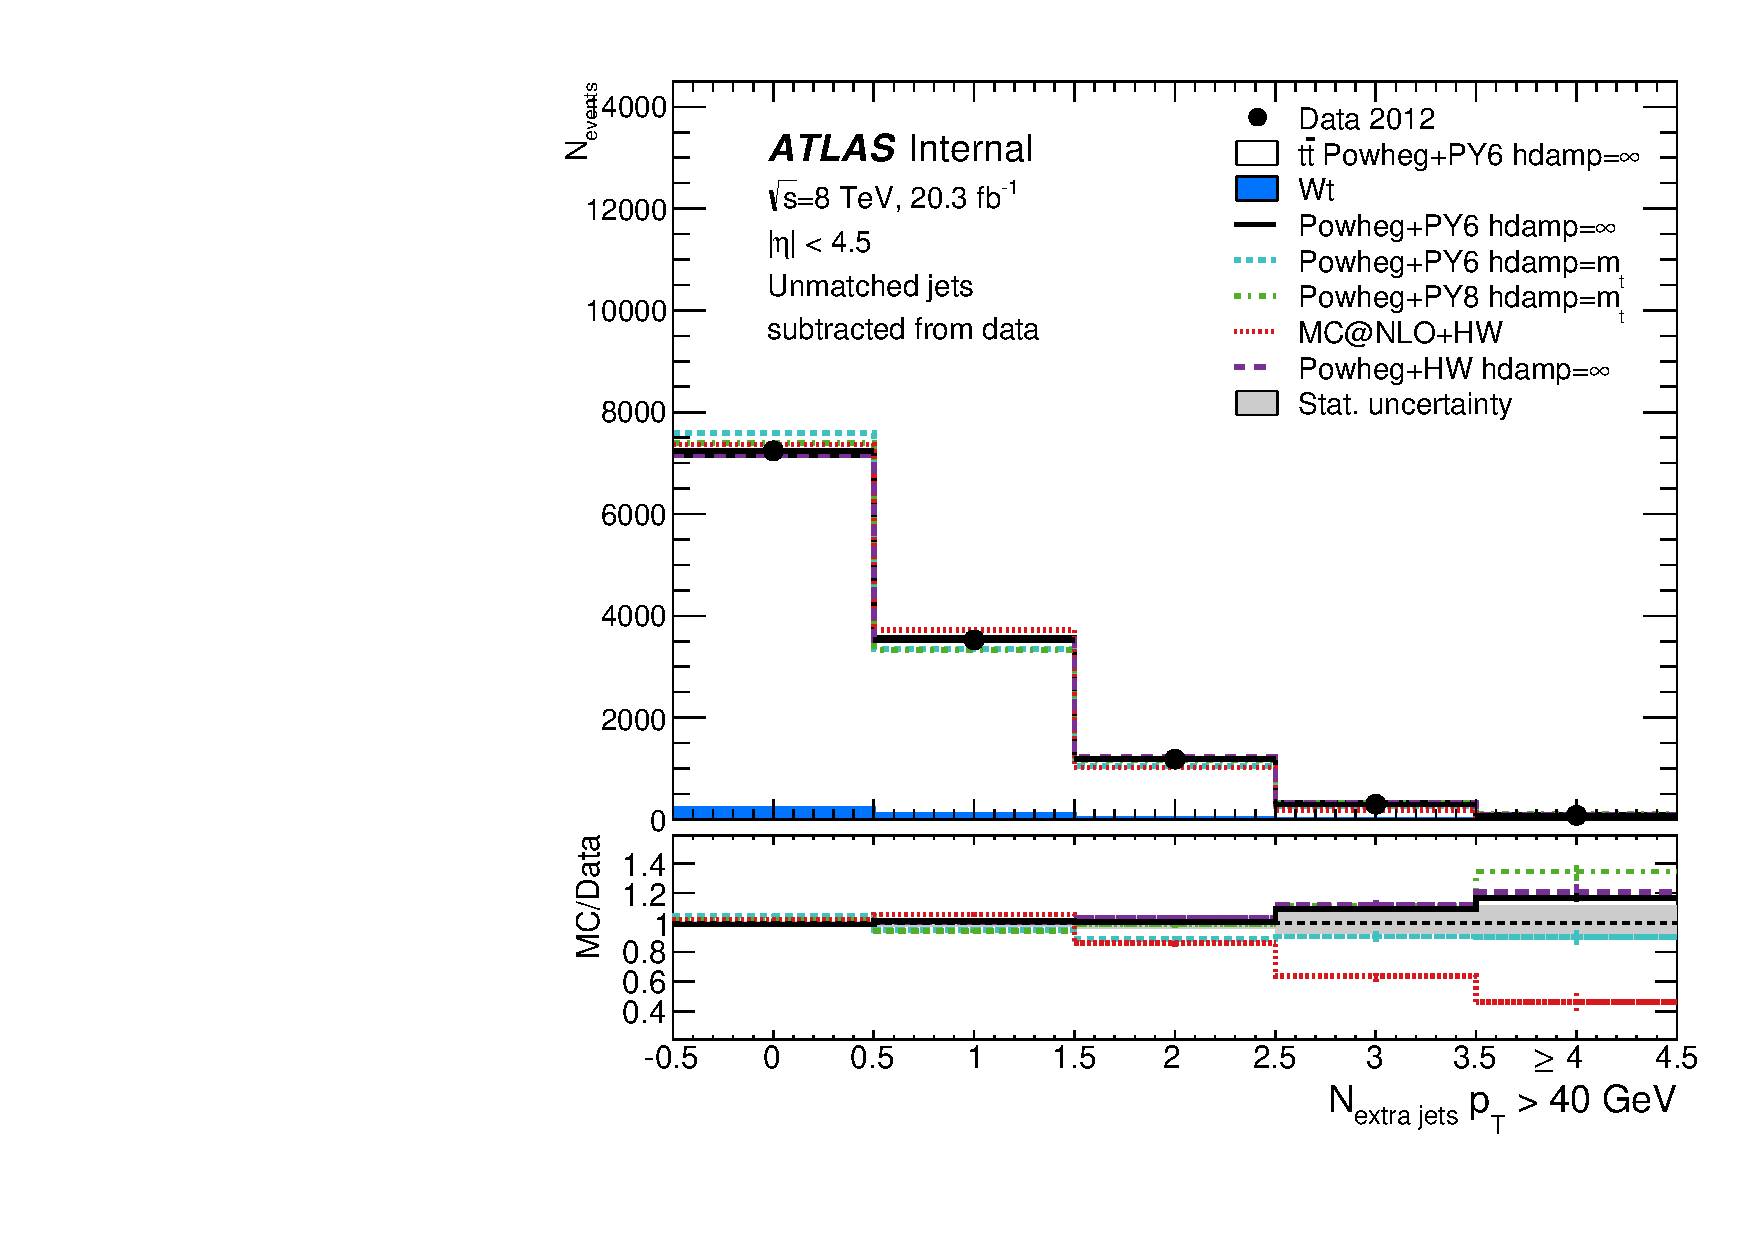
\includegraphics[width=0.45\textwidth]{fig/MCComp/NLO/NExtraJets40NoPileup.pdf}}
\subfloat{
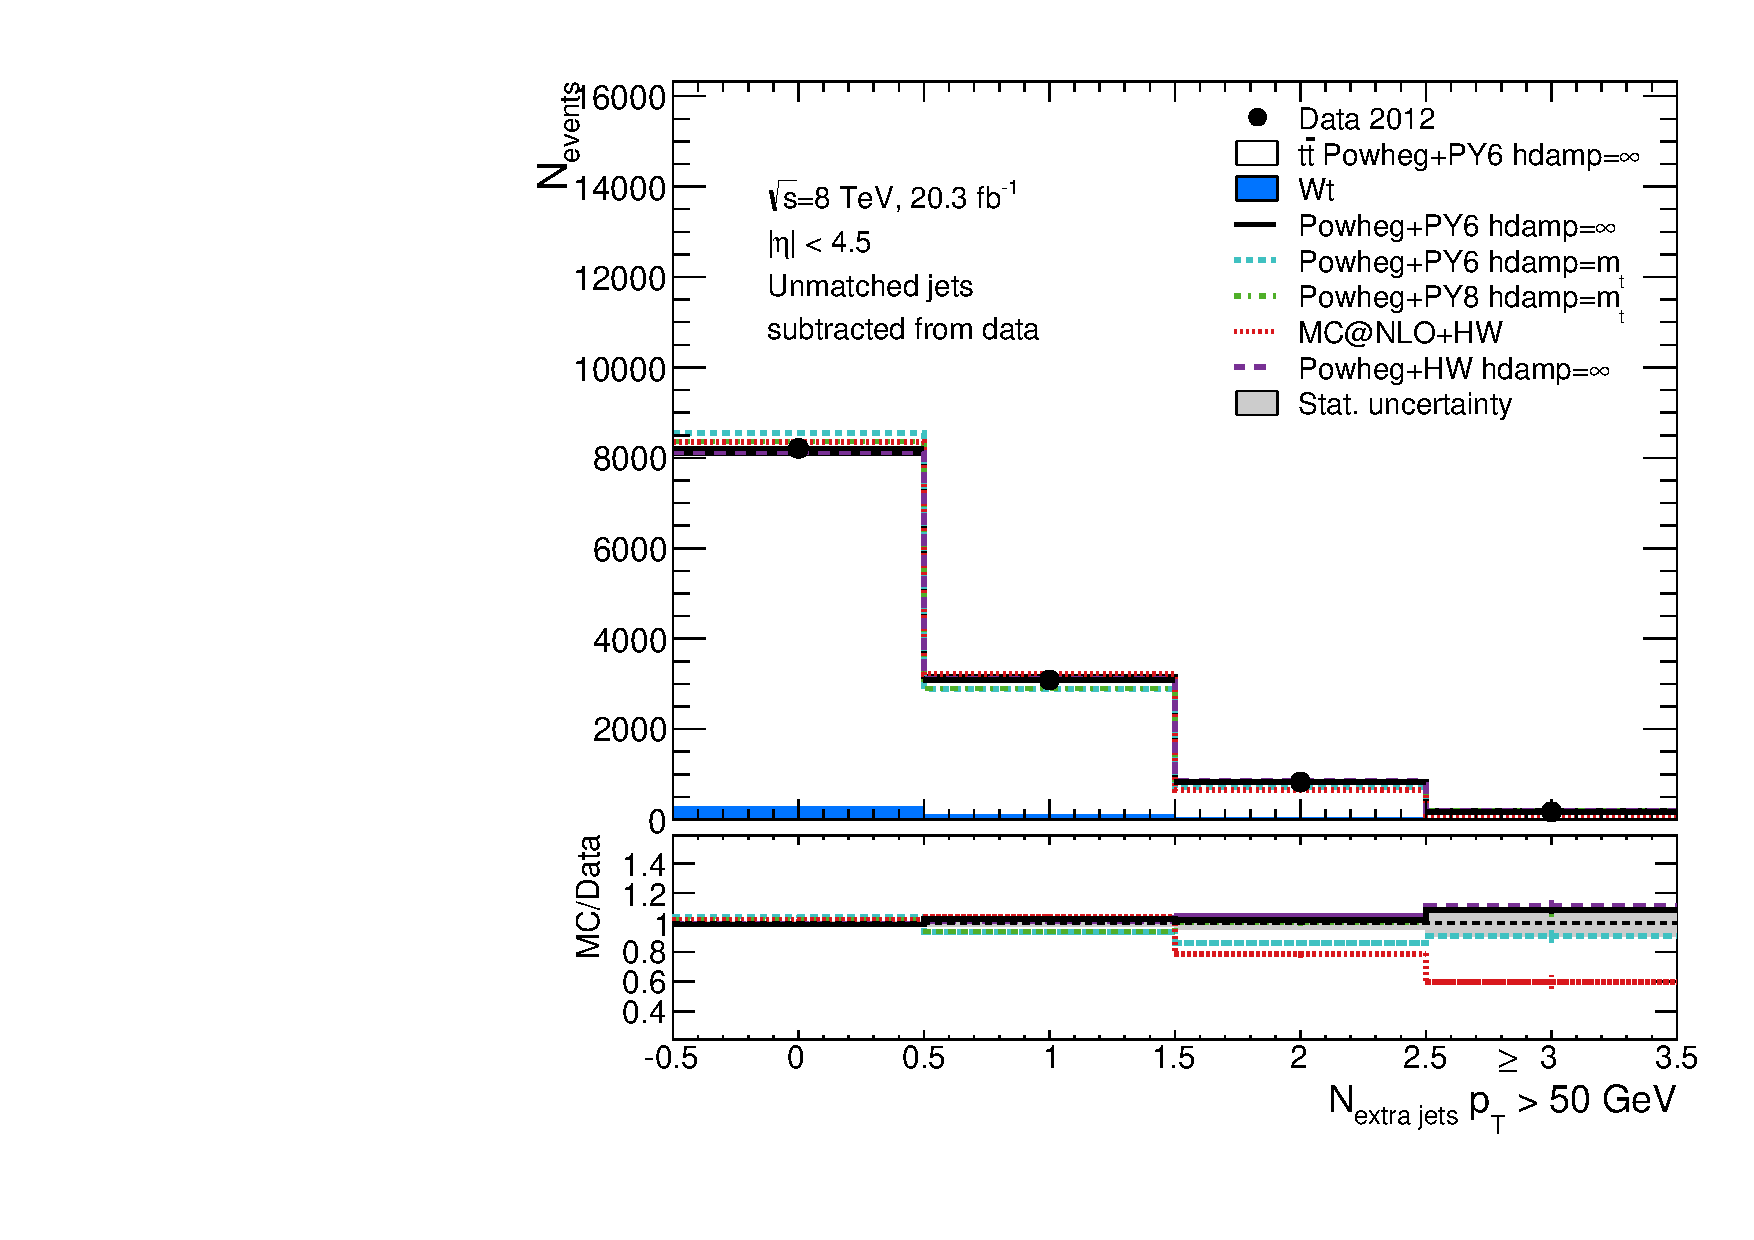
\includegraphics[width=0.45\textwidth]{fig/MCComp/NLO/NExtraJets50NoPileup.pdf}}
\caption{Distributions of the reconstructed extra jet multiplicity as a function of \pt threshold in simulation and data. The distributions in data are compared to \ttbar simulation normalized to the same number of events as in the data. Extra jets from pileup are excluded in simulation by requiring a match to truth. Extra pileup jets are subtracted from the data. The ratio of different MC samples to data is shown with error bars corresponding to the MC statistical uncertainty and a shaded band corresponding to the data statistical uncertainty. Systematic uncertainities are not shown.}
\label{fig:nrecojets}
\end{figure}


\begin{figure}
\centering
\subfloat{
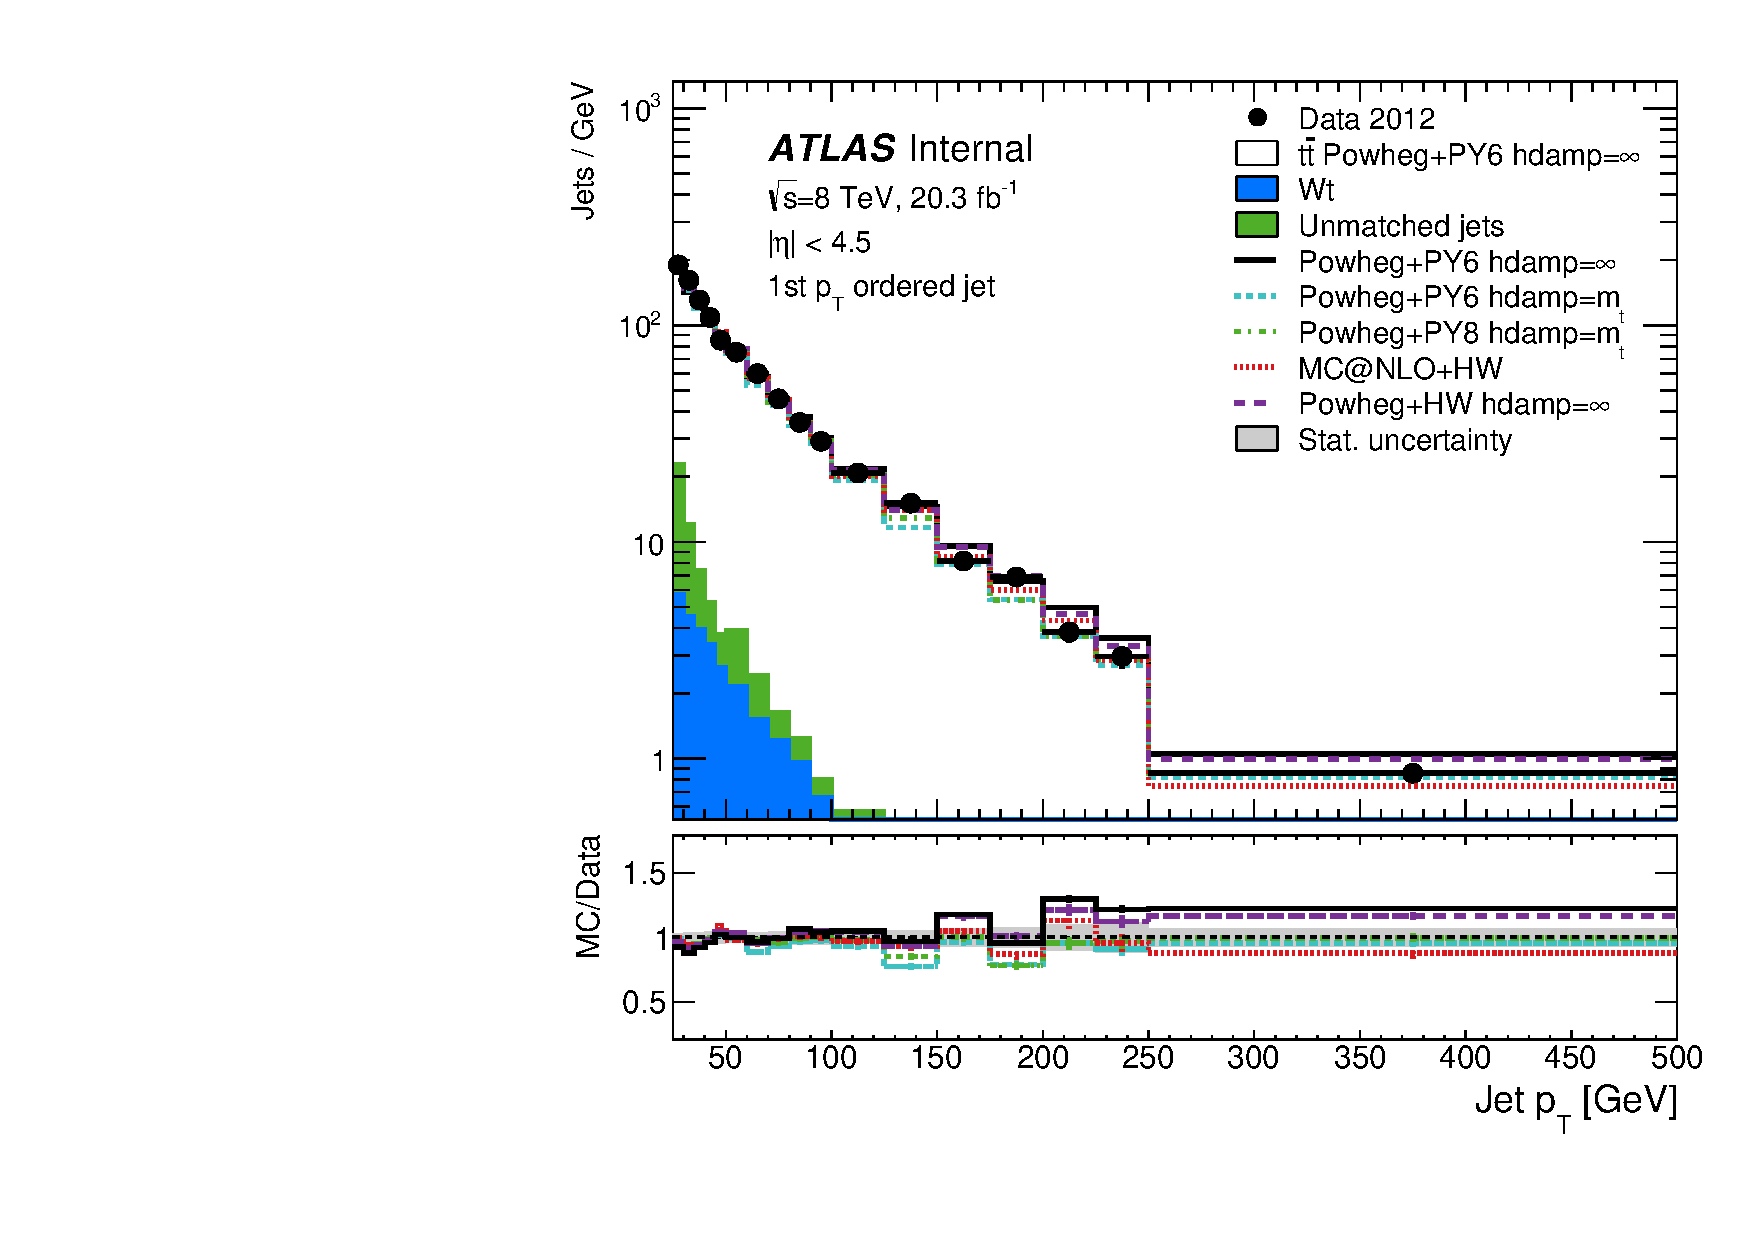
\includegraphics[width=0.45\textwidth]{fig/MCComp/NLO/RecoPtJet0.pdf}}
\subfloat{
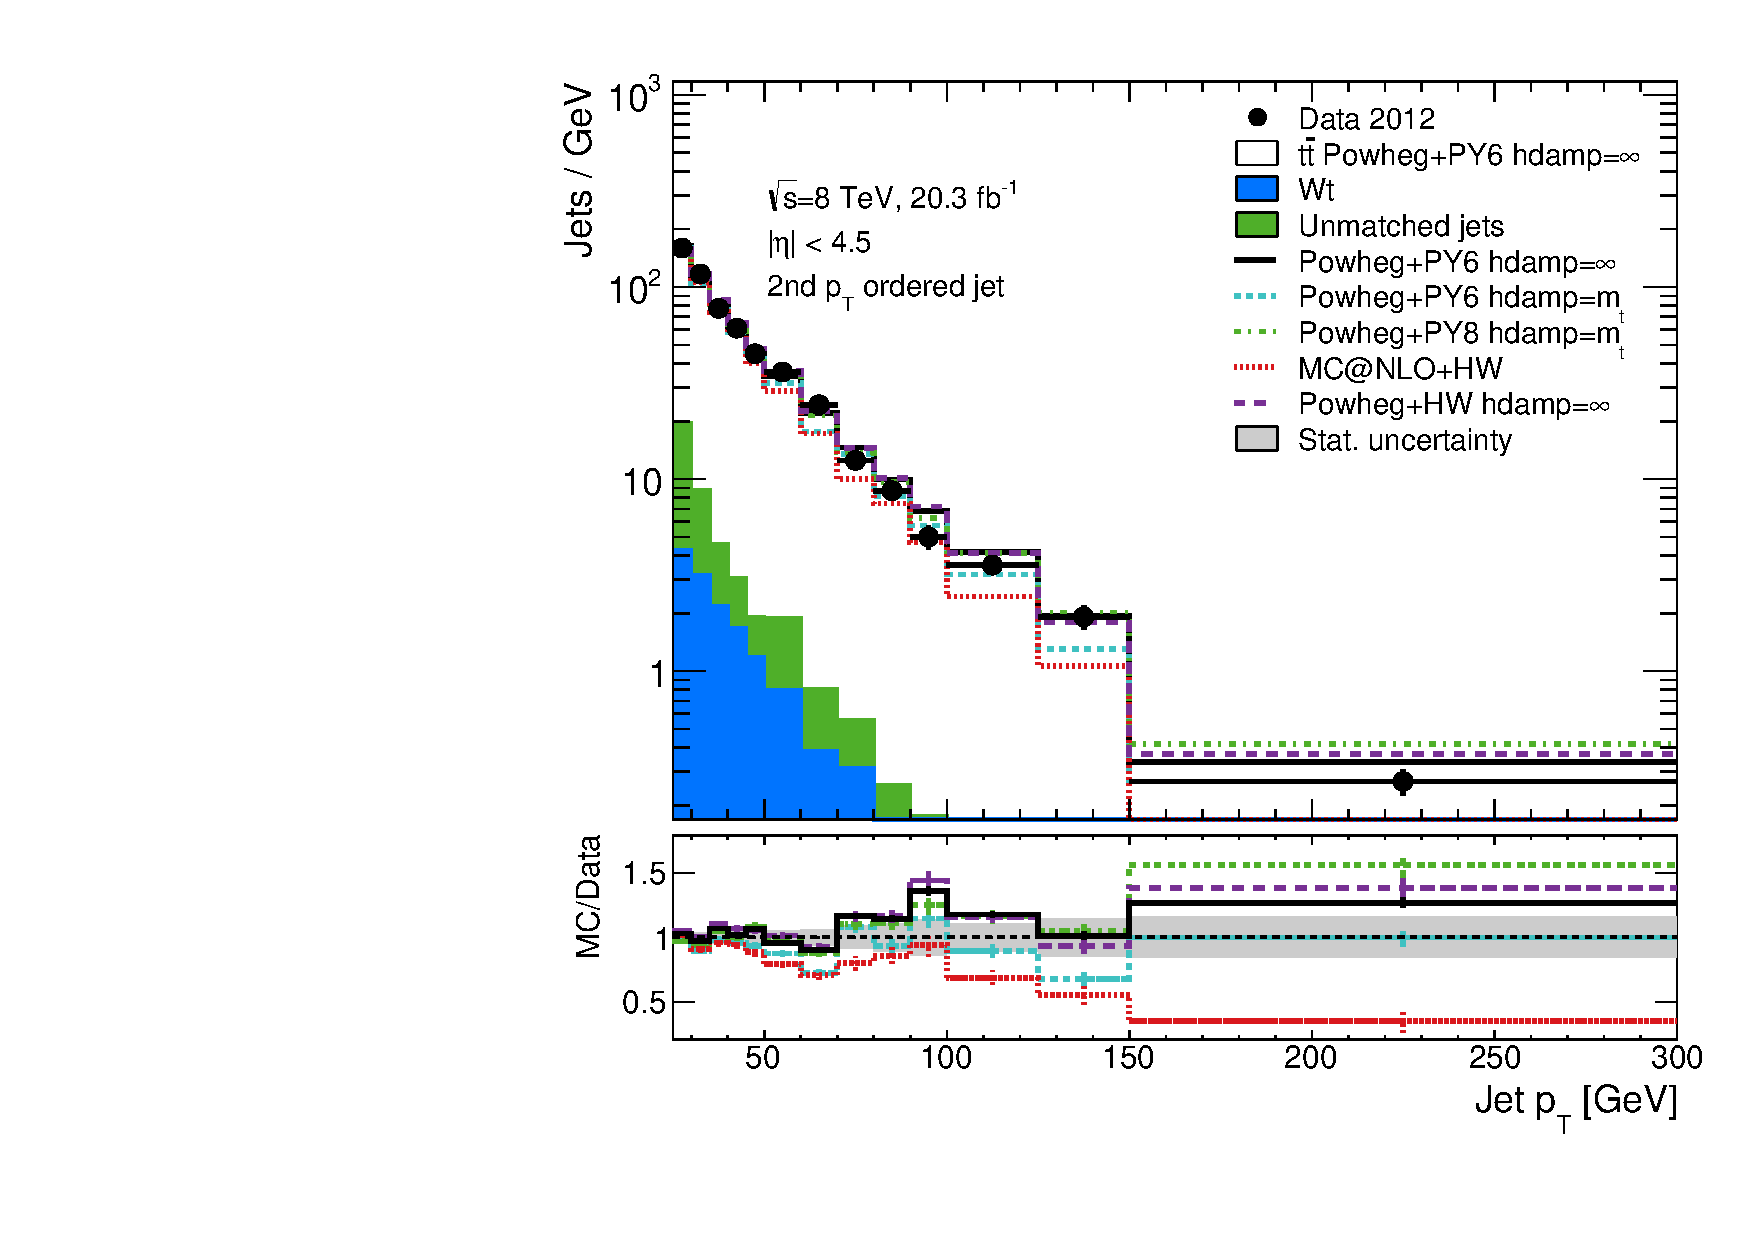
\includegraphics[width=0.45\textwidth]{fig/MCComp/NLO/RecoPtJet1.pdf}}
\\
\subfloat{
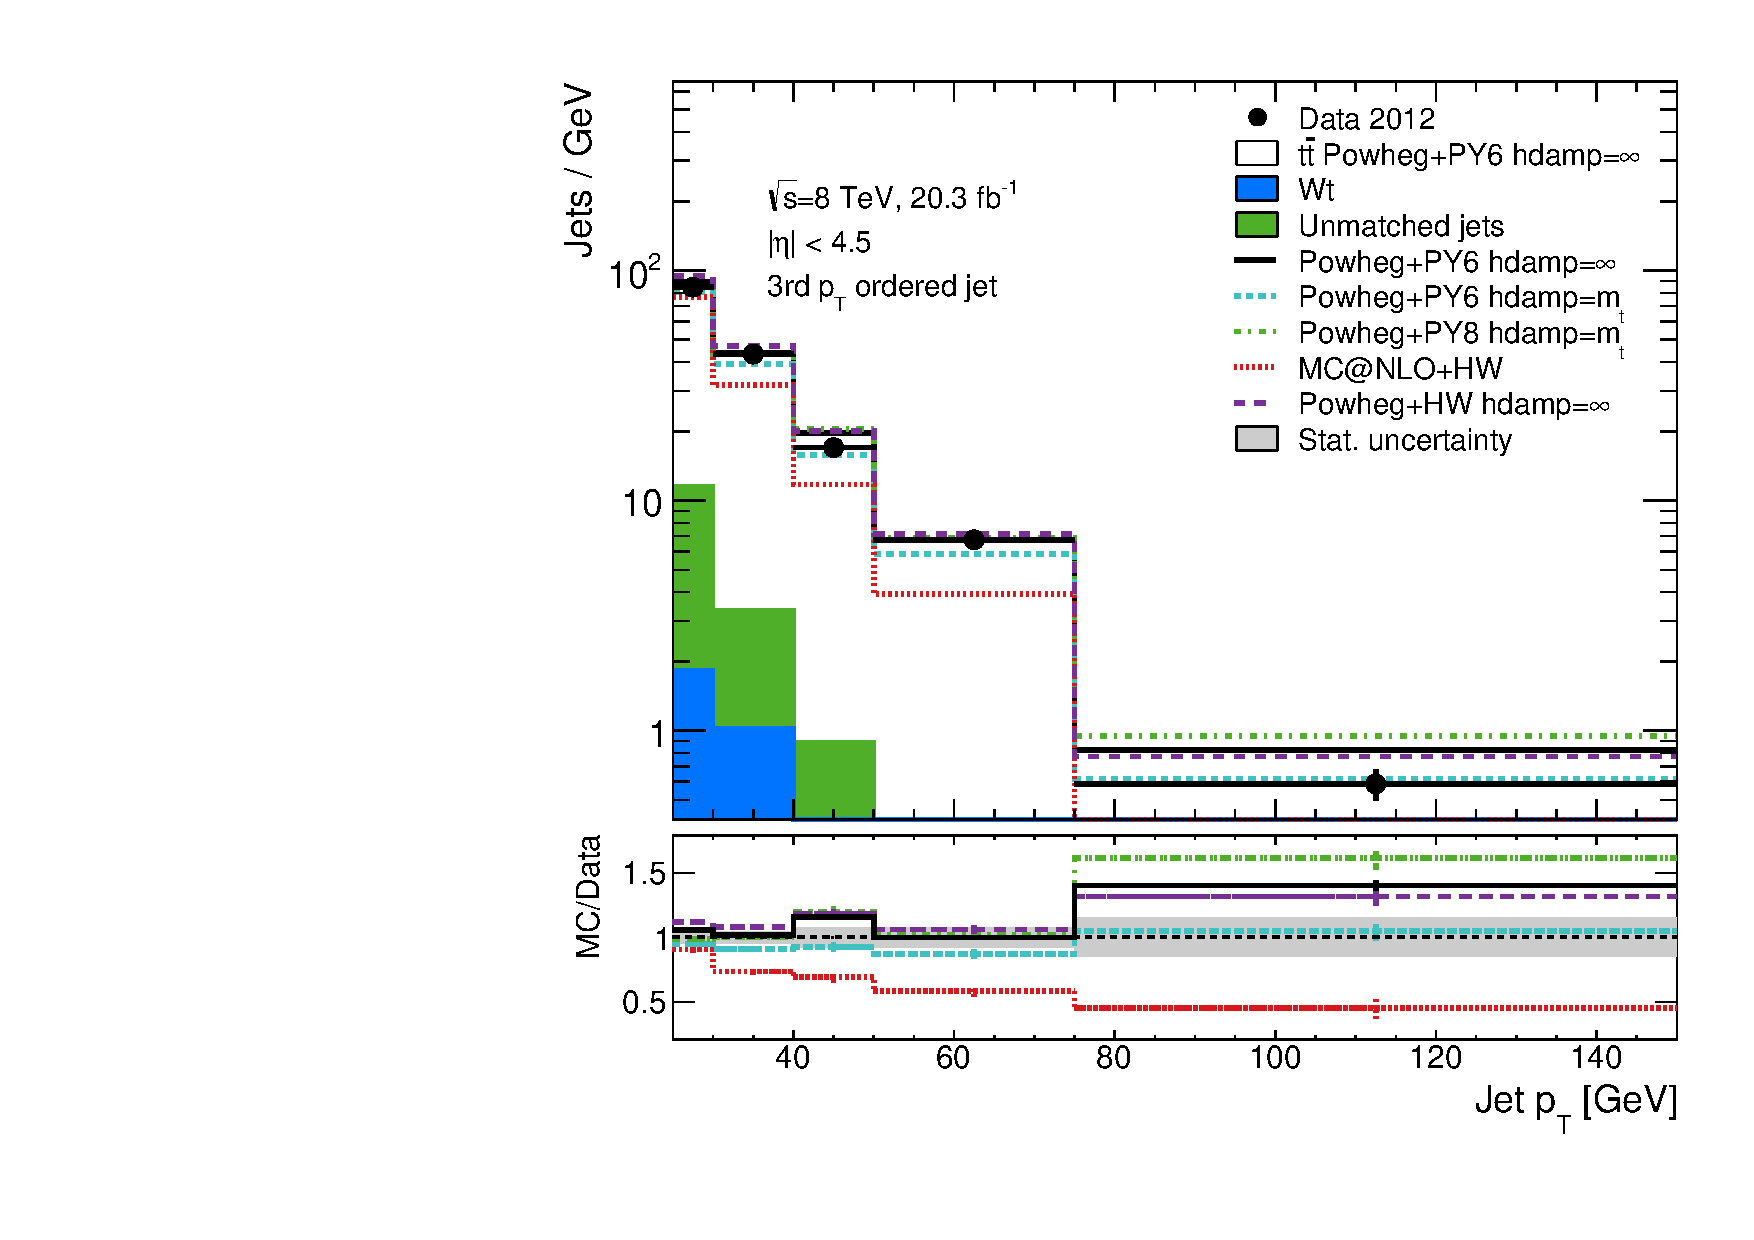
\includegraphics[width=0.45\textwidth]{fig/MCComp/NLO/RecoPtJet2.pdf}}
\subfloat{
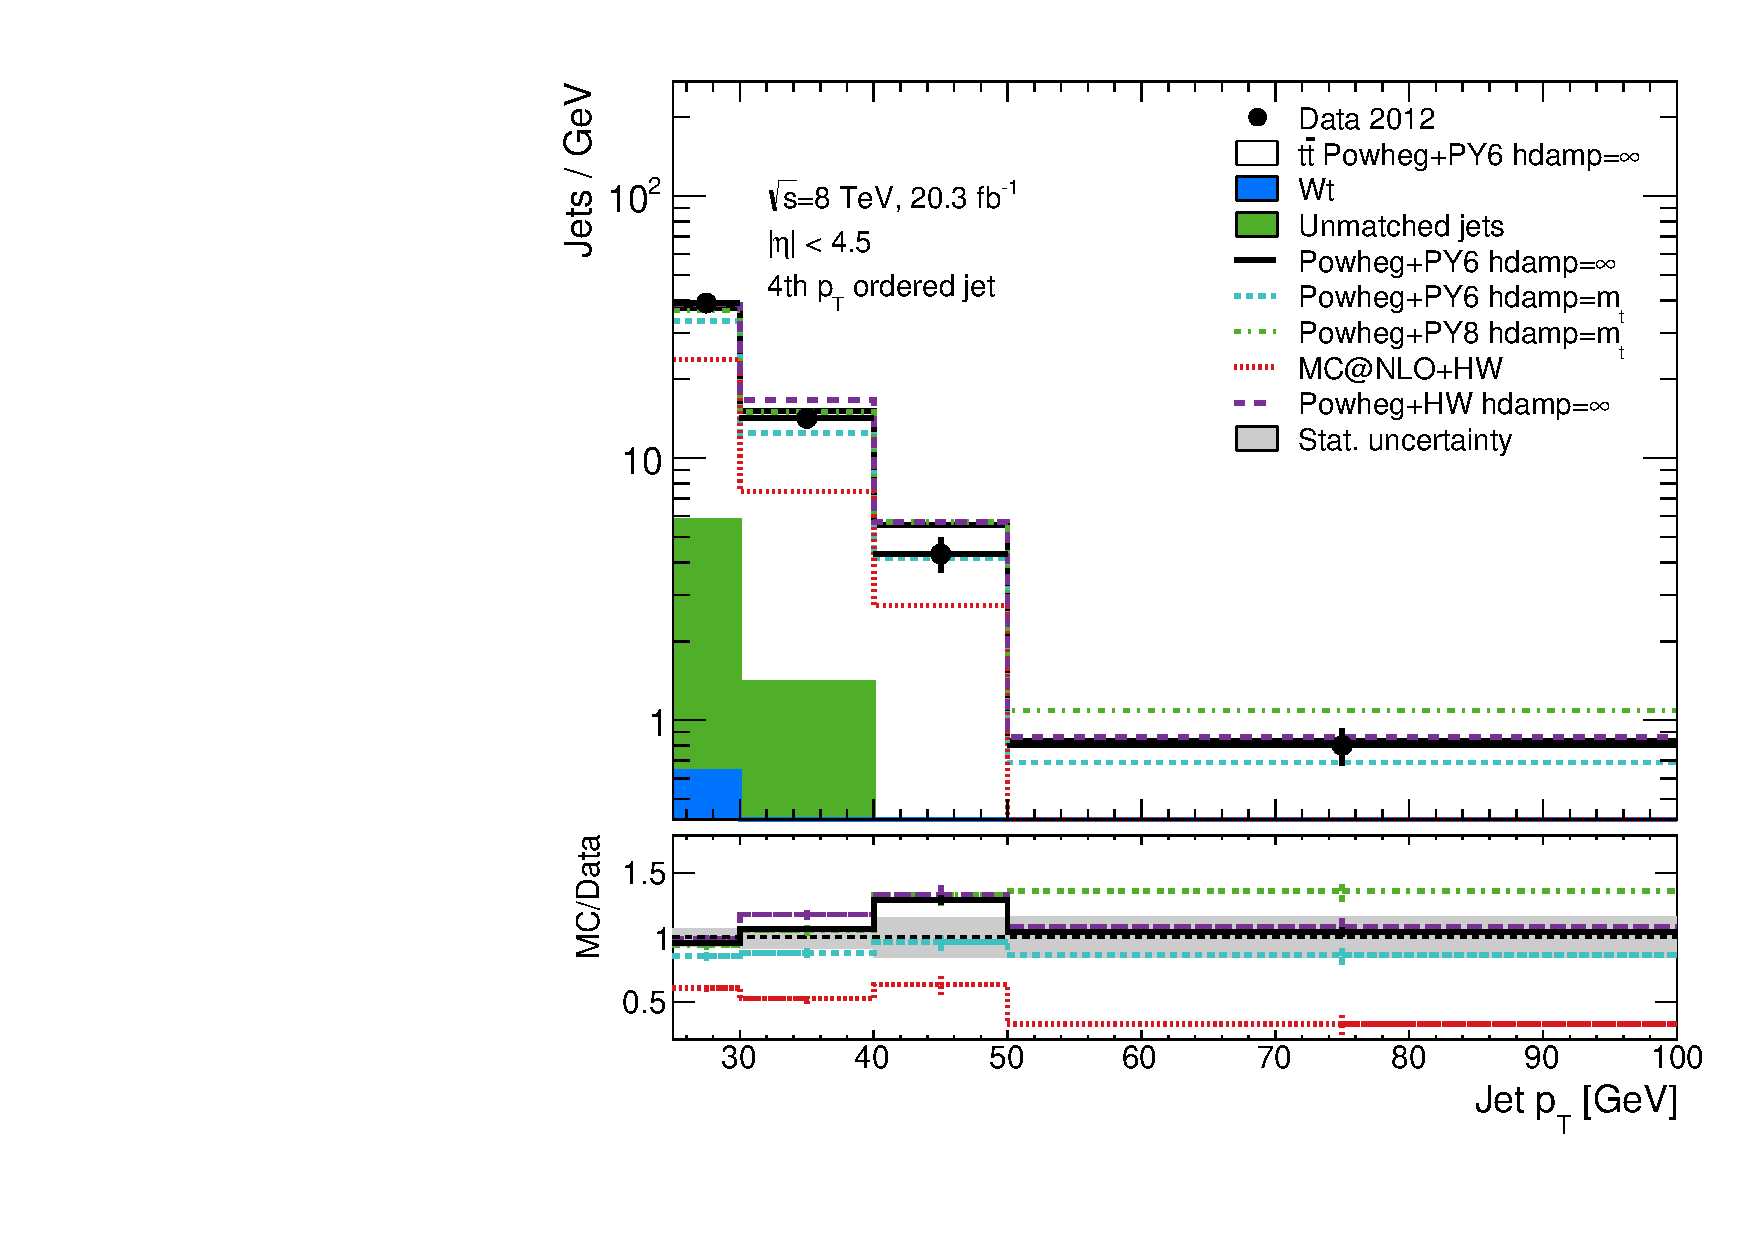
\includegraphics[width=0.45\textwidth]{fig/MCComp/NLO/RecoPtJet3.pdf}}
\caption{Distributions of reconstructed extra jet \pt in simulation and data. The distributions in data are compared to \ttbar simulation normalized to the same number of events as in the data. Backgrounds from single top and extra pileup jets are included as background to \ttbar. The ratio of different MC samples to data is shown with error bars corresponding to the MC statistical uncertainty and a shaded band corresponding to the data statistical uncertainty. Systematic uncertainities are not shown.}
\label{fig:recojetpt}
\end{figure}

